\documentclass[%
 reprint,
 amsmath,amssymb,
 aps,
 pre,
]{revtex4-2}

\usepackage{graphicx}% Include figure files
\usepackage{dcolumn}% Align table columns on decimal point
\usepackage{bm}% bold math
\usepackage{physics}              % Physics notation (bra-ket, diff, etc.)
\usepackage{xcolor}               % Color management
\usepackage{tcolorbox}            % Colored boxes
\usepackage{multirow}
\usepackage{float}
\usepackage{setspace}
\usepackage{enumerate}

% =========================================
%    Algorithms
% =========================================
\usepackage[ruled,linesnumbered]{algorithm2e}
\SetKw{KwContinue}{continue}
\SetKw{KwBreak}{break}

% =========================================
%    Theorems and Proofs
% =========================================
\usepackage{amsthm}
\newtheorem{lemma}{Lemma}
\newtheorem{theorem}{Theorem}
\newtheorem{remark}{Remark}
\newtheorem*{definition}{Definition}

% =========================================
%    Hyperlinks
% =========================================
\usepackage[colorlinks,linkcolor=red!90!black,citecolor=green!75!black]{hyperref}

% =========================================
%    Custom Commands
% =========================================
\newcommand{\setzero}{\setlength{\itemsep}{0pt}}

% Math Operators
\DeclareMathOperator{\KL}{KL}
\DeclareMathOperator{\Var}{Var}
\DeclareMathOperator{\ESS}{ESS}
\DeclareMathOperator{\CESS}{CESS}

% Shortcuts
\newcommand{\D}{\mathrm{d}} 
\newcommand{\Ge}{\geqslant}
\newcommand{\Le}{\leqslant}
\newcommand{\T}{\top}
\newcommand{\ep}{\varepsilon}
\newcommand{\di}{\displaystyle}
\newcommand{\vp}{\varphi}
\newcommand{\JFlow}{\texttt{JeffereysFlow}}

\begin{document}

\title{Jeffreys Flow: Robust Boltzmann Generators for Rare Event Sampling via Distillation of Parallel Tempering}

\author{Guang Lin}
\author{Christian Moya}
\author{Di Qi}
\author{Xuda Ye}
\email{ye481@purdue.edu}
\affiliation{Purdue University, Department of Mathematics, West Lafayette, IN 47907, USA}

\date{\today}

\begin{abstract}
Sampling physical systems with rough energy landscapes is fundamentally limited by rare events and metastable trapping. While generative Boltzmann generators offer a path forward, their reliance on the reverse Kullback--Leibler divergence frequently induces catastrophic mode collapse. Here, we introduce the Jeffreys Flow, a robust generative framework that mitigates this failure by distilling empirical sampling data from Parallel Tempering trajectories using the symmetric Jeffreys divergence. This formulation intrinsically balances local target-seeking precision with global mode coverage. We rigorously prove that minimizing this symmetrized objective suppresses mode collapse and structurally corrects inherent inaccuracies within the finite empirical reference data. We demonstrate the framework's superior scalability and accuracy on highly non-convex multidimensional benchmarks, including the systematic correction of stochastic gradient biases in Replica Exchange SGLD and the massive acceleration of exact importance sampling in Path Integral Monte Carlo for quantum thermal states.
\end{abstract}

\maketitle

\section{Introduction}
\label{section: introduction}

Rare event sampling represents a central challenge in statistical mechanics and computational physics~\cite{bucklew2004introduction, rubino2009rare, rubino2009introduction}. Specifically, consider a target distribution $\pi(x) \propto e^{-U(x)}$ on $\mathbb{R}^d$, where the potential function $U(x)$ exhibits multiple local modes separated by high energy barriers. Classical Monte Carlo methods, such as Metropolis--Hastings, Hamiltonian Monte Carlo (HMC), and Langevin dynamics, routinely suffer from pathologically poor performance, as generated samples become overwhelmingly trapped within a few localized basins. The fundamental difficulty is mathematically formalized by the Eyring--Kramers formula~\cite{eyring1935activated, kramers1940brownian}, which dictates that the transition probability between metastable modes decays exponentially fast with respect to the height of the intervening energy barrier~\cite{bouchet2016generalisation, lee2022non}, inherently rendering such transitions as \emph{rare events} for vanilla Monte Carlo methods.

To simulate the rare events, numerous enhanced Monte Carlo methods have been developed. Representative approaches include Umbrella Sampling~\cite{torrie1977nonphysical, virnau2004calculation, kastner2011umbrella}, Simulated Annealing~\cite{van1987simulated, bertsimas1993simulated, nikolaev2010simulated}, Sequential Monte Carlo (SMC)~\cite{doucet2001introduction, cappe2007overview, chopin2020introduction, wills2023sequential}, Transition Path Sampling~\cite{dellago2002transition}, Metadynamics~\cite{laio2002escaping}, and Parallel Tempering (PT)~\cite{earl2005parallel, miasojedow2013adaptive, syed2022non, deng2023non}. Among these, PT is widely adopted, largely due to its conceptual simplicity and the ease with which it can be implemented in standard simulation codebases. The core mechanism of PT involves simulating multiple replicas of the system in parallel across a defined temperature ladder, ranging from high to low temperatures. By enabling frequent configuration swapping between adjacent replicas, PT allows local low-temperature simulations to mathematically inherit the global ergodicity and rapid state exploration inherent to the high-temperature limits.

Another highly promising approach for sampling complex target distributions relies on flow-based generative models. Empowered by the rapid advancement of GPU architectures, these methods employ a sequence of invertible normalizing flows to pushforward a simple base distribution $\pi_0(x)$ towards the target distribution $\pi(x)$. This framework, known as the Boltzmann generator, was systematically established in the seminal work of \cite{noe2019boltzmann}. The training of a Boltzmann generator is conceptually straightforward and primarily relies on minimizing the reverse Kullback--Leibler (KL) divergence. Formally, this involves finding a sequence of mappings $F$ that minimizes $D_{\text{KL}}(F_{\#} \pi_0 \| \pi)$, where $F_{\#} \pi_0$ denotes the pushforward distribution. In practice, the flow $F$ is parameterized using expressive architectures such as RealNVP~\cite{dinh2016density} or Neural Spline Flows~\cite{durkan2019neural}.

During the inference stage, a trained Boltzmann generator possesses distinct advantages over classical Monte Carlo methods. It circumvents repeated evaluations of the potential gradient, instead leveraging the high memory bandwidth of GPUs to instantly generate massive batches of statistically independent samples. Most importantly, Boltzmann generators ensure theoretically unbiased estimates by employing a straightforward importance sampling reweighting scheme.

Although Boltzmann generators~\cite{noe2019boltzmann, wu2020stochastic} are widely applied in computational physics~\cite{wirnsberger2020targeted,abbott2023normalizing,kohler2024transferable,coretti2024boltzmann,schebek2025scalable}, their reliability in rare event sampling depends heavily on the loss function. When the target distribution $\pi(x)$ contains multiple metastable modes separated by high energy barriers, the pushforward samples of the trained flow are highly prone to becoming trapped in a local basin, entirely missing other significant modes. This phenomenon, known as \emph{mode collapse}~\cite{midgley2022flow, midgley2023learning}, remains the core challenge in designing efficient algorithms for rare event sampling.

\begin{figure}
    \centering
    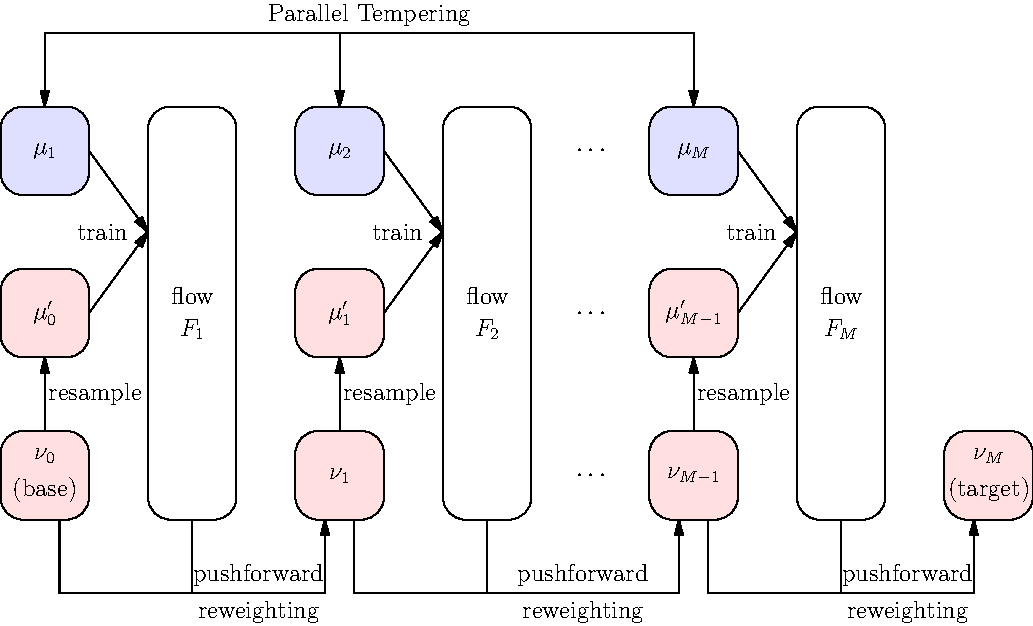
\includegraphics[width=0.5\textwidth]{asy/jeffreys.pdf}
    \caption{The overall architecture of the Jeffreys Flow. PT acts as the principal guide across the temperature ladder, providing reference samples ($\mu_1, \dots, \mu_M$) to train the sequence of normalizing flows ($F_1, F_2, \dots, F_M$). Simultaneously, intermediate states ($\nu_0, \nu_1, \dots, \mu_M$) are progressively pushed forward and reweighted, intrinsically averting mode collapse without relying solely on the target potential function.}
    \label{figure: architecture}
\end{figure}

In this paper, we propose the Jeffreys Flow, a Boltzmann generator specifically tailored for rare event sampling. As the name suggests, the Jeffreys Flow adopts the Jeffreys divergence (i.e., the symmetric KL divergence) as its loss function. Because computing the forward KL divergence requires samples from the target distribution, our method utilizes reference samples generated via PT to train the normalizing flow. In this sense, the Jeffreys Flow can be viewed as effectively distilling the sampling knowledge from PT. Like standard Boltzmann generators, the Jeffreys Flow maintains the benefits of generating statistically independent samples and enabling unbiased reweighting. Most importantly, rather than forcing the flow to learn the complex landscape solely from the target potential, the Jeffreys Flow directly incorporates target samples, thereby successfully avoiding the pervasive issue of mode collapse. For a comprehensive visual overview of this generative distillation architecture, we refer the reader to Figure~\ref{figure: architecture}.

It is worth noting that a variant of the Jeffreys divergence has previously been applied in the original Boltzmann Generator framework~\cite{noe2019boltzmann}. However, it was primarily utilized as a cold-start heuristic in the early stages of training using a small, limited set of target samples, while the core model optimization continued to rely overwhelmingly on the reverse KL divergence. In stark contrast, the Jeffreys Flow treats the reliable samples generated by PT not merely as an initialization aid, but as the principal guide throughout the entire training process. Crucially, despite the seemingly high computational cost of obtaining such reference samples via PT, it is an entirely affordable and worthwhile investment: it provides a profound theoretical guarantee to effectively train the normalizing flow across complex, multimodal landscapes. Once the training is complete, the expensive PT simulation can be entirely discarded, allowing the trained flow to instantaneously generate statistically independent novel samples across the entire predefined temperature ladder in just a few computational steps.

Beyond its intuitive design, the Jeffreys Flow is supported by stringent theoretical guarantees. On the one hand, Theorem~\ref{theorem: correct} establishes that the pushforward distributions $(\nu_k)$ generated by minimizing the Jeffreys divergence are strictly closer to the target distribution than the empirical reference samples $(\mu_k)$, underscoring the capacity of the Jeffreys Flow to intrinsically correct inaccuracies inherent in the PT samples. On the other hand, Theorem~\ref{theorem: concentration} derives a rigorous concentration inequality showing that the probability of mode collapse diminishes to an arbitrarily small level when the Jeffreys divergence is sufficiently minimized. Together, these analytical results confirm that the Jeffreys Flow provides a principled and direct mechanism to prevent mode collapse.

In our numerical experiments, we first showcase the superior performance of the Jeffreys Flow on standard benchmarks up to 16 dimensions. We then extend the framework to two highly challenging applications. First, we integrate the Jeffreys Flow with Replica Exchange Stochastic Gradient Langevin Dynamics (reSGLD)~\cite{deng2020accelerating,li2023fast,lin2023b} for finite-sum potentials. By training the flow on approximate reSGLD samples, we introduce an importance weighting mechanism that systematically corrects the stochastic gradient bias and enhances target accuracy. Second, we apply the Jeffreys Flow to Path Integral Monte Carlo (PIMC)~\cite{herman1982path,marx1996ab,ceriotti2010efficient,schoof2011configuration} for quantum thermal sampling. To circumvent the prohibitive cost of computing full-frequency ring-polymer potentials across a PT ladder, we train a dimensionality-truncated flow solely on the low-frequency normal modes. Exact importance sampling over the full-frequency potential is then performed exclusively at the final step, achieving massive computational acceleration.

\section{Related Works}
\label{section: related works}

To resolve mode collapse in Boltzmann generators, numerous methods directly modify the target loss function away from the vanilla reverse KL. For instance, \cite{falkner2023conditioning} introduces a conditional reverse KL constrained by predefined reaction coordinates, while \cite{dibak2022temperature} trains a single reverse KL-based flow parameterized by continuous temperature. Adaptive annealing strategies are also common: \cite{wang2025mitigating} utilizes the Effective Sample Size (ESS) to dynamically update the temperature ladder, and \cite{matthews2022continual} integrates the reverse KL into Sequential Monte Carlo (SMC) frameworks. Furthermore, \cite{qiu2024efficient} explicitly replaces the reverse KL with the $L^2$-Wasserstein distance between probability densities. While these approaches aim to force the flow to autonomously learn the multi-modal target distribution (often relying heavily on ESS to control the tempering ladder), an alternative strategy abandons the reverse KL entirely in favor of the forward KL~\cite{gabrie2022adaptive, abernethy2024flow}. Although forward KL-based methods exhibit strong mode-covering behavior, they inherently lack the precise physical accuracy provided by energy-based objectives.

Ultimately, Parallel Tempering (PT)~\cite{earl2005parallel, syed2022non} remains the gold standard for handling the rare event sampling. While it may require a significant number of replicas across different temperatures and lacks a bias-correction mechanism such as importance weighting, its efficacy relies primarily on monitoring and maintaining a contiguous swapping rate of approximately 20\% to 40\%. Consequently, if the computational cost of training a normalizing flow vastly exceeds that of PT (for example, when the network size scales poorly with dimensionality or requires an excessive number of flow steps), the flow-based approach loses its practical advantage.

Consequently, the Jeffreys Flow is not designed to supersede PT; instead, it leverages PT samples from both the base and target distributions to directly guide the training of the normalizing flow.
In machine learning terminology, this constitutes a \emph{distillation} procedure aimed at achieving superior efficiency and accuracy in sample generation. The concept of distillation has seen wide application in generative modeling---particularly in image processing and large language models~\cite{luhman2021knowledge, zhou2024simple, xie2024distillation, fu2025moflow}---where it is typically predicated on Score-Based Diffusion~\cite{song2021maximum, batzolis2021conditional} or Flow Matching~\cite{lipman2022flow, chen2023flow}. By contrast, the Jeffreys Flow relies on a straightforward combination of the forward and reverse KL divergences, which is namely the Jeffreys divergence, to construct its loss function.

At this stage, we emphasize that the Jeffreys divergence is not a novel concept; it has already been widely adopted in statistical inference~\cite{moreno2003kullback, bayarri2008generalization, yao2011symmetric, sharma2021clustering} and image processing~\cite{nishii2006image, han2020active}. By symmetrizing the KL divergence, it establishes a stable, pseudo-metric measure that inherently balances the local mode-seeking precision of the reverse KL with the global mass-covering properties of the forward KL, effectively preventing bias from arbitrary directional choices. Consequently, the Jeffreys divergence emerges as a highly promising loss function for flow-based rare event sampling methods.

\section{Single-Step Jeffreys Flow}

In this section, we formalize the training of a single normalizing flow $F:\mathbb{R}^d \to \mathbb{R}^d$ that maps a base distribution $\pi_0(x) \propto e^{-U_0(x)}$ to a target distribution $\pi_1(x) \propto e^{-U_1(x)}$, such that $F_{\#} \pi_0 = \pi_1$. Since the exact continuous distributions $\pi_0$ and $\pi_1$ are intractable, we assume access to their underlying potential functions $U_0(x)$ and $U_1(x)$, alongside empirical reference distributions $\mu_0$ and $\mu_1$ that approximate $\pi_0$ and $\pi_1$. Under this setting, we construct a robust training objective utilizing the Jeffreys divergence, and mathematically demonstrate its superiority over the pure forward and reverse KL divergences.

\subsection{Construction of Jeffreys Divergence}

Since our goal is to achieve $F_{\#} \pi_0 = \pi_1$, minimizing the KL divergence between these two distributions is the most natural choice for the loss function. For instance, considering the reverse KL divergence $D_{\KL}(F_\#\pi_0\|\pi_1)$, the probability density of the pushforward distribution $F_{\#} \pi_0$ is explicitly given by
\begin{equation}
	(F_\# \pi_0)(y) = \frac{\pi_0(x)}{|\det \nabla F(x)|},\quad y = F(x).
	\label{eq: Fpi density}
\end{equation}
Substituting \eqref{eq: Fpi density} into the KL divergence and omitting intractable normalizing constants, we obtain
\begin{align*}
	D_{\KL}(F_\#\pi_0\|\pi_1) &= \mathbb E_{X_0 \sim \pi_0} \Big[ U_1(F(X_0)) - U_0(X_0) \\
	&\quad - \log|\det\nabla F(X_0)| \Big].
\end{align*}
Finally, by replacing the exact base distribution $\pi_0$ with its empirical approximation $\mu_0$, we derive the tractable loss function
\begin{align}
	D_{\KL}(F_\#\pi_0\|\pi_1) &\approx \mathbb E_{X_0 \sim \mu_0} \Big[ U_1(F(X_0)) - U_0(X_0) \notag \\
	&\quad - \log|\det\nabla F(X_0)| \Big],
	\label{eq: rKL}
\end{align}
which crucially does not require any samples from the target distribution $\pi_1$.

Similarly, the forward KL divergence is derived as
\begin{align}
	D_{\KL}(\pi_1\|F_\#\pi_0) 
	&\approx \mathbb E_{X_1 \sim \mu_1} \Big[ U_0(F^{-1}(X_1)) - U_1(X_1) \notag \\
	&\quad - \log|\det\nabla F^{-1}(X_1)| \Big],
	\label{eq: fKL}
\end{align}
which solely requires samples from the target approximate distribution $\mu_1$, entirely bypassing $\pi_0$. 

The Jeffreys divergence is then formulated as a linear combination of the reverse and forward KL divergences:
\begin{equation}
	\mathcal L_J[F] = \lambda_0 D_{\KL}(F_\#\pi_0\|\pi_1) + \lambda_1 D_{\KL}(\pi_1\|F_\#\pi_0),
	\label{eq: Jdiv}
\end{equation}
where $\lambda_0$ and $\lambda_1$ are weighting hyperparameters for the reverse and forward KL. The flow $F$ is parameterized using the Neural Spline Flow architecture~\cite{durkan2019neural}.

Furthermore, we note that the KL divergence components in the loss function~\eqref{eq: Jdiv} can be replaced with the Rényi divergence $D_\alpha(P\|Q)$ to further enhance the robustness of the model against mode collapse. Unlike the standard KL divergence, which relies on the logarithmic expectation $\mathbb E_P[\log(P/Q)]$, the Rényi divergence is governed by the power-law moment $\mathbb E_P[(P/Q)^{\alpha-1}]$, recovering the KL divergence exactly in the limit as $\alpha \to 1$. This scaling mechanism intrinsically assigns amplified gradients to extreme particles situated in the isolated modes or distribution tails. Therefore, we recommend adopting the Rényi objective when a sufficiently large number of training samples is available to stabilize the high-variance weights, as it fosters a more comprehensive coverage of complex multimodal target landscapes.

\subsection{Jeffreys Divergece Mitigates Mode Collapse}

While the reverse KL divergence $D_{\KL}(F_\#\pi_0\|\pi_1)$ is theoretically capable of generating high-fidelity samples, it is intrinsically prone to mode collapse. This critical limitation arises because the reverse KL is inherently mode-seeking; if the generated distribution $F_\#\pi_0$ captures only a localized subset of the modes of $\pi_1$ while ignoring others, the associated divergence penalty remains negligible.

In contrast, incorporating the forward KL effectively mitigates mode collapse. The divergence $D_{\KL}(\pi_1\|F_\#\pi_0)$ strongly penalizes missing mass, growing unbounded if the generated distribution $F_\#\pi_0$ fails to adequately cover any region where the target $\pi_1$ holds substantive probability. However, training a flow exclusively utilizing the forward KL presents its own challenge: because computing the forward KL relies on the empirical approximation $\mu_1$, the fidelity of $F_\#\pi_0$ becomes strictly bottlenecked by the accuracy of $\mu_1$ relative to the true target $\pi_1$.

To provide a rigorous theoretical analysis of the generated sample quality, we simplify the setting by assuming that the empirical base distribution is exact, i.e., $\mu_0 = \pi_0$, while $\mu_1$ remains an imperfect approximation of $\pi_1$. Under this assumption, the Jeffreys divergence $\mathcal L_J[F]$ defined in \eqref{eq: Jdiv} evaluates exactly to
\begin{equation*}
	\mathcal L_J[F] = \lambda_0 D_{\KL}(F_\#\pi_0\|\pi_1) + 
	\lambda_1 \mathbb E_{X_1\sim \mu_1} 
	\bigg[\log\frac{\pi_1(X_1)}{F_\#\pi_0(X_1)}\bigg].
\end{equation*}
Expressing $\mathcal L_J[F]$ explicitly via the pushforward density $P(x) = (F_\#\pi_0)(x)$, we derive the simplified functional
\begin{equation*}
	\mathcal L_J[P] =  \lambda_0 \int P(x) \log \frac{P(x)}{\pi_1(x)}\D x + \lambda_1 \int \mu_1(x)\log \frac{\pi_1(x)}{P(x)}\D x.
\end{equation*}
Noting that $\int \mu_1(x) \log \pi_1(x)\D x$ is a constant independent of $P$, we can equivalently identify the functional as
\begin{equation}
	\mathcal L_J[P] = \lambda_0 D_{\KL}(P\|\pi_1) + \lambda_1 D_{\KL}(\mu_1\|P) + \mathrm{const}.
	\label{eq: LJP}
\end{equation}

In the limiting case of pure forward KL (i.e., $\lambda_0 \to 0$), it is straightforward to observe that the unique global minimizer is trivially $P_*(x) = \mu_1(x)$. Consequently, a flow trained exclusively via the forward KL is inherently bottlenecked by the quality of the empirical samples, preventing the approximation error from decreasing below the intrinsic error of $\mu_1$. However, by utilizing the Jeffreys divergence, we establish the following rigorous theoretical guarantees regarding sample quality:
\begin{theorem}
\label{theorem: correct}
Assuming the weighting parameters satisfy $\lambda_0, \lambda_1 > 0$, the following hold true:
\begin{enumerate}
	\setlength{\itemsep}{4pt}
	\item The functional $\mathcal L_J[P]$ is strictly convex with respect to the density $P$, ensuring the existence of a unique global minimizer $P_*$.
	\item The unique minimizer $P_*$ satisfies the divergence bound $D_{\KL}(P_*\|\pi_1 ) \Le D_{\KL}(\mu_1\|\pi_1)$.
\end{enumerate}
\end{theorem}
\mbox{}
\begin{proof}
For the first claim, we begin by computing the second-order derivative of $\mathcal L_J[P]$ with respect to $P$:
\begin{equation*}
	\frac{\delta^2 L_J}{\delta P^2}(x) = \frac{\lambda_0}{P_1(x)} + 
	\frac{\lambda_1 \mu_1(x)}{P^2(x)} > 0,
\end{equation*}
which immediately demonstrates that $\mathcal L_J[P]$ is strictly convex with respect to $P$. Therefore, $\mathcal L_J[P]$ admits a unique global minimizer $P_*$. Noting that the first-order functional derivative is given by
\begin{equation*}
	\frac{\partial L_J}{\partial P} = \lambda_0 \log \frac{P(x)}{\pi_1(x)}
	- \frac{\lambda_1 \mu(x)}{P(x)} + \mathrm{const},
\end{equation*}
we find that the optimal density $P_*$ is intrinsically determined by the system of equations
\begin{equation*}
\left\{
\begin{aligned}
	\lambda_0 \log \frac{P_*(x)}{\pi_1(x)}
	- \frac{\lambda_1 \mu(x)}{P_*(x)} & = c_*, \\
	\int P(x) \D x & = 1,
\end{aligned}
\right.
\end{equation*}
where $c_*\in\mathbb R$ represents a normalization constant. 

Regarding the second claim, the optimality condition trivially implies $\mathcal L_J[P_*] \Le \mathcal L_J[\mu_1]$. Substituting this into the alternative expression~\eqref{eq: LJP} gives
\begin{equation*}
\lambda_0 D_{\KL}(P_*\|\pi_1) + \lambda_1 D_{\KL}(\mu_1\|P_*) \Le 
\lambda_0 D_{\KL}(\mu_1\|\pi_1 ).
\end{equation*}
Since $D_{\KL}(\mu_1\|P_*)\Ge 0$, we immediately obtain the bound
\begin{equation*}
	\lambda_0 D_{\KL}(P_*\|\pi_1) \Le 
	\lambda_0 D_{\KL}(\mu_1\|\pi_1 ),
\end{equation*}
which yields the desired result.
\end{proof}

Theorem~\ref{theorem: correct} establishes that the generated pushforward distribution $P_* = F_\#\pi_0$ strictly bounds the KL divergence achieved by the empirical reference $\mu_1$. This fundamental inequality essentially proves that a flow trained via the Jeffreys divergence guarantees a closer approximation to the true target $\pi_1$ than the training data $\mu_1$ itself can provide. This distillation capability is rooted in the synergistic nature of the loss function: while the forward KL efficiently resolves the mode collapse issue by firmly anchoring the generative support onto the diverse empirical modes of $\mu_1$, the reverse KL simultaneously acts as an exact physics-based regularizer. By directly penalizing deviations against the true potential $U_1$, the reverse KL continuously refines the pushforward density and robustly corrects intrinsic finite-sample errors and noise from the reference data.

Moreover, the Jeffreys divergence offers a rigorous theoretical guarantee regarding the boundedness of the likelihood ratio. Let $P$ and $Q$ be two probability measures on $\mathbb R^d$ with strictly positive densities $P(x)$ and $Q(x)$. We define the $\delta$-instability set $A_\delta$ as the region where the log-likelihood ratio exceeds a threshold $\delta$:
\begin{equation}
	A_\delta = \bigg\{x\in\mathbb R^d:
	\bigg|\log \frac{P(x)}{Q(x)}\bigg| \Ge \delta
	\bigg\}.
\end{equation}
The following lemma establishes that minimizing the Jeffreys divergence  bounds the probability mass of $A_\delta$. For related probability bounds under specified divergences, see the literature on density ratio estimation~\cite{sugiyama2012density} and the Bretagnolle--Huber inequality~\cite{tsybakov2008nonparametric}.
\begin{lemma}
	\label{lemma: concentration}
	Assume the distributions $P$ and $Q$ satisfy $D_{\KL}(P\|Q) \Le \epsilon$ and $D_{\KL}(Q\|P) \Le \epsilon$. Then the probability measure of the instability set $A_\delta$ is bounded by
	\begin{equation}
		\max\big(P(A_\delta),Q(A_\delta)\big) \Le \frac{2\ep}{\delta(1-e^{-\delta})}.
		\label{eq: mPQb}
	\end{equation}
\end{lemma}
\begin{proof}
By definition, the KL divergence bounds yield
\begin{equation}
\int_{\mathbb R^d} (P(x) - Q(x))\log\frac{P(x)}{Q(x)} \D x \Le 2\epsilon.
\label{eq: PQep}
\end{equation}
Note that the integrand in \eqref{eq: PQep} is completely nonnegative. We partition the instability set $A_\delta$ into
\begin{equation*}
	S_+ = \{P(x) \Ge e^\delta Q(x)\}, \quad S_- = \{Q(x) \Ge e^\delta P(x)\},
\end{equation*}
and denote their respective contributions to the integral \eqref{eq: PQep} by $I_+$ and $I_-$. Thus, $I_++I_-\Le 2\epsilon$.

On $S_+$, we have $\log\frac{P(x)}{Q(x)} \Ge \delta$ and
\begin{equation*}
	I_+ \Ge \int_{S_+} P(x)(1-e^{-\delta})\delta \D x = \delta(1-e^{-\delta})P(S_+).
\end{equation*}
Since $Q(x) \Le P(x)$ on $S_+$, we find
\begin{equation}
	Q(S_+) \Le P(S_+) \Le \frac{I_+}{\delta(1-e^{-\delta})}.
	\label{eq: QPd}
\end{equation}
By symmetry, on $S_-$ we obtain
\begin{equation}
	P(S_-) \Le Q(S_-) \Le \frac{I_-}{\delta(1-e^{-\delta})}.
	\label{eq: PQd}
\end{equation}
Since $I_++I_-\Le 2\ep$, adding \eqref{eq: QPd} and \eqref{eq: PQd} yields \eqref{eq: mPQb}.
\end{proof}

Applying Lemma~\ref{lemma: concentration} directly to our context where $P = F_\# \pi_0$ and $Q = \pi_1$ yields the following main result regarding the sample quality of the pushforward distribution.

\begin{theorem}
\label{theorem: concentration}
Given the continuous distributions $\pi_0$ and $\pi_1$,
suppose the flow $F$ satisfies $D_{\KL}(F_\#\pi_0\|\pi_1) \Le \epsilon$ and $D_{\KL}(\pi_1\|F_\#\pi_0) \Le \epsilon$. For any $\delta > 0$, the probability that the log-likelihood deviates by more than $\delta$ is bounded by:
\begin{align}
	\mathbb{P}_{X\sim F_\#\pi_0} \bigg( \bigg| \log \frac{F_\#\pi_0(X)}{\pi_1(X)} \bigg| & \Ge \delta \bigg) 
	\Le \frac{2\epsilon}{\delta(1 - e^{-\delta})},	\\
 \mathbb{P}_{Y\sim \pi_1} \bigg( \bigg| \log \frac{F_\#\pi_0(Y)}{\pi_1(Y)} \bigg| & \Ge \delta \bigg) \Le \frac{2\epsilon}{\delta(1 - e^{-\delta})}.
\end{align}
\end{theorem}
Theorem~\ref{theorem: concentration} guarantees that with high probability, the generated distribution $F_\#\pi_0$ and the target $\pi_1$ are mutually absolutely continuous with bounded density ratios. Consequently, this prevents mode collapse (where $\pi_1 \gg F_\#\pi_0$) and spurious mode generation (where $F_\#\pi_0 \gg \pi_1$) asymptotically as the training error $\epsilon \to 0$.

\mbox{}

\subsection{Unbiased Estimation via Importance Sampling}

While the trained flow $F$ models the optimal transport between distributions, it rarely yields an exact mapping where $F_\#\pi_0 = \pi_1$. Nevertheless, we can systematically recover unbiased estimators for expectations under the target $\pi_1$ through importance sampling. The statistical reliability of this estimation relies on the absolute continuity of the generated distribution with respect to the target, requiring that the flow must adequately cover the entirety of the support of $\pi_1$ without mode collapse.

Recall that the density of the pushforward distribution is evaluated exactly via the change-of-variable formula:
\begin{equation*}
	(F_\#\pi_0)(y) = \frac{\pi_0(x)}{|\det \nabla F(x)|}, \quad y =F(x).
\end{equation*}
Consequently, we define the unnormalized importance weight $w(y)$ as the likelihood ratio between the target and the generated distributions:
\begin{equation}
	w(y) = \frac{\pi_1(y)}{(F_\#\pi_0)(y)} \propto e^{- U_1(y) + U_0(x) + \log|\det \nabla F(x)|}.
\end{equation}
The intractable partition functions are omitted as they readily cancel out during self-normalized importance sampling. Notice that the weight $w(y)$ corresponds exactly to the likelihood ratio whose stability is rigorously bounded in Theorem~\ref{theorem: concentration}. If the pushforward density $F_\#\pi_0$ drops probability mass in regions where $\pi_1(y)$ remains substantial, the corresponding weights $w(y)$ inevitably diverge or exhibit unbounded variance.

For notational convenience, we abstract the single-step Jeffreys Flow operation as:
\begin{equation*}
(F, w) = \mathtt{JeffreysFlow}(\mu_0 , \mu_1 ; U_0 , U_1 ).
\end{equation*}
This notation encapsulates the entire procedure: training the transport map $F$ using the empirical
samples $\mu_0$, $\mu_1$ and potential functions $U_0$, $U_1$, and subsequently computing the importance weights $w$. In particular, the quality of the optimized flow $F$ can be quantitatively assessed using the Conditional Effective Sample Size (CESS):
\begin{equation}
	\CESS(F,w) = \frac{\big(\int_{\mathbb R^d} w(y) \mu_0(F^{-1}(y))\D y\big)^2}{\int_{\mathbb R^d} w^2(y) \mu_0(F^{-1}(y))\D y},
\end{equation}
which lies in $[0,1]$ due to Cauchy's inequality. CESS also serves as the standard metric in SMC~\cite{doucet2001introduction} for evaluating sample degeneracy, where a value approaching $1$ indicates high sample quality.

More generally, for a discrete empirical distribution
\begin{equation*}
	\mu_0(x) = \sum_{i=1}^N \alpha_i \delta(x-x_i),\quad 
	\text{where} ~
	\sum_{i=1}^N \alpha_i = 1,
\end{equation*}
its Effective Sample Size (ESS) is defined as
\begin{equation}
	\ESS(\mu_0) = \frac{\big(\sum_{i=1}^N \alpha_i\big)^2}{N\sum_{i=1}^N \alpha_i^2} \Le 1.
\end{equation}
In the specific case where $\mu_0$ is an empirical distribution with uniform weights,
\begin{equation*}
	\mu_0(x) = \frac{1}{N} \sum_{i=1}^N \delta(x-x_i),
\end{equation*}
and $\mu_1 = F_\# \mu_0$, the CESS of the flow $F$ simplifies to
\begin{equation*}
	\CESS(F,w) = \frac{\big(\sum_{i=1}^N w(y_i)\big)^2}{N\sum_{i=1}^N w^2(y_i)},\quad \text{with} ~ y_i = F(x_i),
\end{equation*}
which exactly recovers $\ESS(F_\# \mu_0)$.

\subsection{Choice of Hyperparameters \(\lambda_0, \lambda_1\)}

Recall the definition of the Jeffreys divergence in \eqref{eq: Jdiv}:
\begin{equation*}
	\mathcal L_J[F] = \lambda_0 D_{\KL}(F_\#\pi_0\|\pi_1) + \lambda_1 D_{\KL}(\pi_1\|F_\#\pi_0)
\end{equation*}
We employ a variance-based scaling for the weights:
\begin{equation}
	\lambda_0 = \theta \Var(\mu_0), \quad \lambda_1 = (1 - \theta) \Var(\mu_1),
	\label{eq: lambda 01}
\end{equation}
where $\Var(\cdot)$ denotes the trace of the covariance, and $\theta \in [0, 1]$ is a balancing hyperparameter.

By scaling the loss weights according to variance, we implicitly balance their corresponding gradients. When transforming a high-variance source distribution $\mu_0$ into a low-variance target $\mu_1$, the reverse KL divergence provides the necessary geometric constraints to ensure global coverage of the target modes. At the same time, this balanced scaling preserves the fine-grained convergence driven by the forward KL divergence.

While the algorithm generally demonstrates robustness to the choice of $\theta$, excessively large values---which heavily favor the forward KL---can still induce sudden mode collapse, indicated by a sharp decline in the CESS. Therefore, in practice, we select $\theta$ by continuously monitoring the CESS; alternatively, one can simply switch to the R\'enyi divergence to achieve stronger geometric constraints for mode-covering.

\section{Sequential Distillation from Parallel Tempering}

\subsection{Reference Samples from Parallel Tempering}

Given a simple base distribution $\pi_0(x) \propto e^{-U_0(x)}$ such as a Gaussian or uniform distribution, our goal is to efficiently sample from a multi-modal target distribution $\pi_M(x) \propto e^{-U_M(x)}$. Directly training a deterministic flow $F$ to map $\pi_0$ onto $\pi_M$ is often practically infeasible, as it requires $F$ to learn complicated deformations. Moreover, constrained by the topological structure of diffeomorphisms, deterministic flows are prone to establishing artificial bridges between well-separated local modes.

To circumvent this, the standard practice in Boltzmann Generators \cite{noe2019boltzmann} and Stochastic Normalizing Flows (SNF) \cite{wu2020stochastic} is to introduce a temperature ladder to bridge the base and target distributions. Let $M$ be the total number of transitions, and consider the interpolated potential sequence
\begin{equation}
	U_k(x) = \lambda_k U_0(x) + (1-\lambda_k) U_M(x), \quad 0\Le k\Le M,
\end{equation}
where the pacing parameters $\{\lambda_k\}_{k=0}^M$ satisfy
\begin{equation*}
	0 = \lambda_0 < \lambda_1 < \cdots < \lambda_M = 1.
\end{equation*}
This sequence induces $M-1$ intermediate distributions $\pi_k(x) \propto e^{-U_k(x)}$, and decomposes the global generation process into $M$ localized flow transformations $F_k$, each satisfying $(F_k)_\# \pi_{k-1} = \pi_k$. To further avoid the emergence of mode connections, SNF \cite{wu2020stochastic} interleaves stochastic diffusion steps after each deterministic flow layer.

In contrast to vanilla Boltzmann generators, the Jeffreys Flow requires reference samples for each intermediate distribution $\pi_k$. specifically, to train the map $F_k$, we need approximate samples from both $\pi_{k-1}$ and $\pi_k$. In this case, PT \cite{syed2022non} emerges as a natural approach to generate the required training data.

Over the family of distributions $\{\pi_k\}_{k=0}^M$, PT simulates $M+1$ overdamped Langevin dynamics in parallel:
\begin{equation*}
	\D X_k(t) = -\nabla U_k(X_k(t))\D t + \sqrt{2}\D B_k(t),
	\quad 0\Le k\Le M,
\end{equation*}
where $\{B_k(t)\}_{k=0}^M$ are independent Brownian motions in $\mathbb R^d$. 
Although each process $X_k(t)$ admits $\pi_k(x) \propto e^{-U_k(x)}$ as its invariant distribution, the low-temperature samplers suffer from slow mixing times due to high energy barriers.
To enable global ergodicity, PT proposes configuration exchanges between adjacent replicas $X_{k-1}(t) = x_{k-1}$ and $X_k(t) = x_k$. The energy difference associated with this proposed swap is given by
\begin{equation*}
	\Delta H_k = U_{k-1}(x_k) + U_k(x_{k-1}) - U_{k-1}(x_{k-1}) - U_k(x_k).
\end{equation*}
To preserve the detailed balance condition, this proposed exchange is accepted with the Metropolis--Hastings probability $\min\{1, e^{-\Delta H_k}\}$.

PT simulations require all $M+1$ processes $\{X_k(t)\}_{k=0}^M$ simultaneously, and high-accuracy samples usually demands a very small time step. In long-time simulations, this can impose a significant CPU and memory burden. However, in the Jeffreys Flow, we can let PT generate only low-fidelity samples that cover all modes. Once the flow models $\{F_k\}_{k=0}^M$ are trained on these samples, we can utilize the flows to instantly generate a large number of accurate samples from the target distribution $\pi_M$. Notably, monitoring the sampling quality in PT is straightforward: standard practice dictates that an average acceptance rate of 20\%--40\% is typically sufficient to ensure global ergodicity \cite{syed2022non}.

\subsection{Sequential Flow Training Framework}

Next, our goal is to learn a sequence of flows $\{F_k\}_{k=1}^M$ such that $(F_k)_\# \pi_{k-1} = \pi_k$. Assuming PT generates an approximate empirical distribution $\mu_k$ for each $\pi_k$, a natural approach is to use $\mu_{k-1}$ and $\mu_k$ to train the flow $F_k$:
\begin{equation*}
	(F_k, w_k) = \mathtt{JeffreysFlow}(\mu_{k-1} , \mu_k ; U_{k-1} , U_k ).
\end{equation*}
However, because the empirical distributions $\mu_{k-1}$ and $\mu_k$ are inherently biased, the resulting $F_k$ may deviate from the true minimizer of the Jeffreys divergence, leading to a low CESS in the distillation steps.

To address this issue, we employ a more robust sequential training strategy, as described in Fig.~\ref{figure: architecture}. First, we initialize a large ensemble $\nu_0$ from the base distribution $\pi_0\propto e^{-U_0}$. Then at each step $k=1,\dots,M$, we construct a refined empirical distribution $\mu_{k-1}'$ by resampling from the large ensemble $\nu_{k-1}$, and train the flow $F_k$ via
\begin{equation*}
	(F_k, w_k) = \mathtt{JeffreysFlow}(\mu_{k-1}' , \mu_k ; U_{k-1} , U_k ).
\end{equation*}
After the training at each step, we compute the pushforward of $(F_k,w_k)$ on $\nu_{k-1}$ to obtain the updated distribution $\nu_k$. In this manner, each $\nu_k$ theoretically provides an unbiased estimate of $\pi_k$ due to the importance weights, and the final output $\nu_M$ serves as a highly accurate approximation to the target distribution $\pi_M$.

\begin{algorithm*}
\label{algorithm}
\setstretch{1.1}
\caption{Jeffreys Flow: Sequential Distillation from Parallel Tempering}
\KwIn{base potential $U_0$, target potential $U_M$, interpolating parameters $\{\lambda_k\}_{k=0}^M$, reference samples $\{\mu_k\}_{k=0}^M$}
\KwOut{trained flow models $\{F_k\}_{k=0}^M$, high-fidelity samples $\{\nu_k\}_{k=0}^M$}

\tcp{A. Initialization}
Generate samples $\nu_0$ from the base distribution $\pi_0\propto e^{-U_0}$ with uniform weights.

\tcp{B. Flow Distillation}
\For{$k=1,\dots,M$}{
	\tcp{I. Data Preparation}
	Set the target potential $U_k(x) = \lambda_k U_M(x) + (1-\lambda_k) U_0(x)$. \\
	Resample the ensemble $\mu_{k-1}'$ from the source distribution $\nu_{k-1}$. \\
	\emph{(Optional)} Apply Monte Carlo rejuvenation on $\mu_{k-1}'$ to update the positions. \\
	\tcp{II. Flow Optimization}
	Compute the balancing parameters $\lambda_0 = \Var(\mu_{k-1}')$ and $\lambda_1 = \Var(\mu_k)$. \\
	Train the flow $F_k$ and compute the weights $w_k$ by minimizing the Jeffreys divergence defined in \eqref{eq: rKL}--\eqref{eq: Jdiv}:
	\begin{equation*}
		(F_k, w_k) = \mathtt{JeffreysFlow}(\mu_{k-1}' , \mu_k ; U_{k-1} , U_k ).
	\end{equation*}
	
	\tcp{III. Propagation and Reweighting}
	Compute the pushforward and reweighted distribution $\nu_k$:
	\begin{equation*}
		\nu_k = (F_k, w_k)_\# \nu_{k-1}.
	\end{equation*}
	
	\tcp{IV. Adaptive Resampling for low ESS}
	\If{$\ESS(\nu_k)<50\%$}{
		Resample the distribution $\nu_k$ from itself to restore uniform weights.
	}
	\emph{(Optional)} Apply Monte Carlo rejuvenation on $\nu_k$ to update the positions.
}

\tcp{C. Output Results}
Output the trained flow models $\{F_k\}_{k=0}^M$ and the samples $\{\nu_k\}_{k=0}^M$.
\end{algorithm*}

In practice, the sample size of the output ensemble $\nu_k$ can and should be significantly larger than that of the training ensemble $\mu_k$. On the one hand, we require $\nu_k$ to achieve higher statistical accuracy. On the other hand, evaluating the flow pushforward $F_k$ on $\nu_k$ during inference is computationally much cheaper than performing repeated backpropagation on $\mu_k$ during training. Thus, it is computationally reasonable to use this strategy.

For completeness, we present the full pipeline of the Jeffreys Flow in Algorithm~\ref{algorithm}. In addition to the standard procedure described above, we strongly recommend employing rejuvenation steps to improve sample quality. Following the practice in \cite{wu2020stochastic}, at each step $k$, we can apply a few steps of the Metropolis-Adjusted Langevin Algorithm (MALA) to the generated samples $\nu_k$ with respect to the target distribution $\pi_k$, which helps eliminate artificial bridges connecting different modes. Furthermore, we introduce an adaptive resampling strategy where the weighted distribution $\nu_k$ is forcibly resampled whenever its ESS drops below $50\%$, effectively preventing ill-posed output distributions.

\section{Applications in Replica Exchange SGLD}
\label{section: reSGLD}

Many sampling tasks, particularly in Bayesian inference, involve a potential energy function with a finite-sum structure:
\begin{equation}
	U_M(x) = \frac{1}{L} \sum_{i=1}^L V^i(x),
\end{equation}
where $\{V^i(x)\}_{i=1}^L$ is a collection of component potentials in $\mathbb{R}^d$. When the target distribution $\pi_M \propto e^{-U_M}$ is multimodal, designing an efficient and accurate sampling algorithm poses a significant challenge.

The Replica Exchange Stochastic Gradient Langevin Dynamics (reSGLD)~\cite{deng2020accelerating} offers a scalable framework to sample such distributions. To reduce the computational cost of evaluating full gradients, reSGLD employs a mini-batch potential for the PT simulation:
\begin{equation}
	U_k^{\mathcal B}(x) = (1-\lambda_k) U_0(x) + \frac{\lambda_k}{|\mathcal B|} \sum_{i\in\mathcal B} V^i(x),
\end{equation}
where the subset $\mathcal B \subset \{1,\dots,L\}$ is shared across all temperature indices $k=0,1,\dots,M$. Consequently, the Langevin dynamics is replaced by its stochastic variant:
\begin{equation*}
    X_k(t + h) = X_k(t) - h \nabla U_k^{\mathcal B}(X_k(t)) + \sqrt{2h}(B_k(t + h) - B_k(t)),
\end{equation*}
where $\{B_k(t)\}_{k=0}^M$ are independent Brownian motions in $\mathbb{R}^d$. Since the stochastic gradient is unbiased, this numerical scheme is exact in the continuous-time limit $h \to 0$.

However, computing the swapping rate between adjacent replicas presents a core challenge. Using the mini-batch approximation, the stochastic energy difference for swapping configurations $x_{k-1}$ and $x_k$ at pacing parameters $\lambda_{k-1}$ and $\lambda_k$ is
\begin{equation*}
	\Delta H_k^{\mathcal B} = U_{k-1}^{\mathcal B}(x_k) + U_k^{\mathcal B}(x_{k-1}) - U_{k-1}^{\mathcal B}(x_{k-1}) - U_k^{\mathcal B}(x_k),
\end{equation*}
yielding a naive acceptance probability
\begin{equation}
\alpha_k^{\mathcal B} = \min\big\{1, e^{-\Delta H_k^{\mathcal B}}\big\}.
\label{eq: akB}
\end{equation} 
Due to the nonlinearity of the exponential function, \eqref{eq: akB} yields a biased estimator of the true swapping probability, even if $\Delta H_k^{\mathcal B}$ itself remains an unbiased.

To correct the bias from naive energy difference, reSGLD adopts a variance-penalized acceptance criterion:
\begin{equation}
    \alpha_k^{\mathcal B} = \min \left\{ 1, \exp\left(-\Delta H_k^{\mathcal B} - \frac{\tau}{2} \sigma_k^2\right) \right\},
\end{equation}
where $\sigma_k^2\approx \Var(\Delta H_k^{\mathcal B})$ is the empirical variance of the stochastic energy difference, and $\tau \in (0, 1]$ is a fixed hyparameter. This corrected variance formally compensates for the second-order Taylor expansion error of the exponential function, thus improving the accuracy for computing the acceptance probabilities.

Although reSGLD can generate the reference sample $\{\mu_k\}_{k=0}^M$ analogous to standard PT, it inherently sacrifices theoretical exactness in computing the acceptance probablity, even in the limit $h \to 0$. By contrast, the Jeffreys Flow effectively circumvents this limitation---the Jeffreys divergence for training the map $F_k$, defined in \eqref{eq: rKL}--\eqref{eq: Jdiv}, depends linearly on the potential functions $U_{k-1}$ and $U_k$. Consequently, Jeffreys Flow theoretically guarantees the exact transport map $F_k$, requiring however additional training epochs to average out the variance.

After training $F_k$, computing the importance weights using the full exact potential is highly affordable, as it requires only a single  evaluation across the ensemble $\nu_{k-1}$. In contrast, reSGLD demands frequent replica swapping to maintain ergodicity, hence a mini-batch approximation to the energy difference remains essential for efficiency. Furthermore, the Monte Carlo rejuvenation steps in Algorithm~\ref{algorithm} can be implemented via a Stochastic Variance-Reduced Gradient (SVRG) \cite{johnson2013accelerating,reddi2016stochastic} strategy. By initially evaluating the full gradient for the entire ensemble $\nu_k$, this variance reduction technique yields highly accurate gradients, enabling us to safely simulate the Langevin dynamics without Metropolis rejection steps.

Even when evaluating the full potential is computationally prohibitive, we can still perform accurate importance sampling via a residual matching technique. Specifically, we train auxiliary neural networks $\phi$ and $\psi$ by minimizing the $L^2$ loss:
\begin{align*}
    \mathcal{L}_2[\phi, \psi] & = \mathbb{E}_{X_0 \sim \nu_{k-1}} \Big[ \big( U_k^{\mathcal{B}}(F_k(X_0)) - U_{k-1}^{\mathcal{B}}(X_0) \\
    & \hspace{2cm} + \phi(X_0) - \psi(F_k(X_0)) \big)^2 \Big],
\end{align*}
where $U_k^{\mathcal{B}}$ and $U_{k-1}^{\mathcal{B}}$ denote the strictly unbiased mini-batch approximations of the potentials. Upon convergence, we utilize $\psi(y) - \phi(x) - \log |\det \nabla F_k(x)|$ as a surrogate for the intractable log-importance weights $\log w_k(y)$. This surrogate achieves high accuracy because the $L^2$ residual loss provides a significantly finer resolution than the standard KL divergence.

\section{Applications in Path Integral Monte Carlo}

\subsection{Path Integral Formulation}

In Path Integral Monte Carlo (PIMC), the primary objective is to compute quantum thermal averages by sampling a quantum canonical ensemble. Under the path integral formulation~\cite{reed1972methods}, this ensemble is mathematically equivalent to a continuous probability distribution over an infinite-dimensional space of imaginary-time paths.

To formalize this, consider a quantum system in $\mathbb{R}^d$ governed by the Hamiltonian operator:
\begin{equation}
    \hat{H} = -\frac{1}{2} \Delta + V(x),
\end{equation}
where $\Delta$ is the Laplacian and $V: \mathbb{R}^d \to \mathbb{R}$ is the potential energy function. For a system at inverse temperature $\beta$, the density matrix of the thermal Boltzmann ensemble $e^{-\beta \hat{H}}$ exactly corresponds to a probability measure on the space of closed continuous paths $x: [0, \beta] \to \mathbb{R}^d$. This measure is governed by the Euclidean action functional:
\begin{equation}
    U(x(\cdot)) = \int_0^\beta \left( \frac{1}{2} |\dot{x}(t)|^2 + V(x(t)) \right) \D t.
\end{equation}

Here, the kinetic energy term $\frac{1}{2} |\dot{x}(t)|^2$ induces a Gaussian reference measure tying the path into a closed ring, while the potential $V(x(t))$ modifies the local density. The target distribution is thus formally given by:
\begin{equation*}
    \pi(x(\cdot)) \propto e^{-U(x(\cdot))}.
\end{equation*}
Generating samples from this infinite-dimensional measure provides a direct and exact framework for evaluating macroscopic thermodynamic properties.

To computationally sample the infinite-dimensional measure $\pi(x(\cdot))$, we construct a finite-dimensional approximation. By discretizing the imaginary-time interval $[0, \beta]$ into $N$ equal segments, we represent the continuous path as a discrete sequence of beads $x_1, \dots, x_N \in \mathbb{R}^d$ subject to the periodic boundary condition $x_{N+1} = x_1$. The Euclidean action functional is thus approximated by the discrete ring-polymer potential:
\begin{equation}
    U_N(x_{1:N}) = \frac{N}{2\beta} \sum_{j=1}^N |x_j - x_{j+1}|^2 + \frac{\beta}{N} \sum_{j=1}^N V(x_j),
    \label{eq: UNx}
\end{equation}
and the discretized target distribution is now:
\begin{equation*}
	\pi_N(x_{1:N})\propto \exp\big(-U_N(x_{1:N})\big).
\end{equation*}
To decouple the stiff harmonic interactions between adjacent beads, we assume $N$ is even and apply a discrete Fourier transform. This maps the Cartesian coordinates $\{x_k\}_{k=1}^N$ into the normal mode coordinates $\{\xi_k\}_{k=0}^{N-1}$:
\begin{equation}
    \xi_k = \frac{\beta}{N} \sum_{j=1}^N x_j c_{j,k}, \quad k = 0, 1, \dots, N-1.
\end{equation}

Here, the orthogonal transformation matrix elements $c_{j,k}$ are explicitly given by:
\begin{align*}
    c_{j,0} &= \frac{1}{\sqrt{\beta}}, \quad c_{j,N-1} = \frac{(-1)^j}{\sqrt{\beta}}, \\
    c_{j,2k-1} &= \sqrt{\frac{2}{\beta}} \sin\left(\frac{2\pi k j}{N}\right), \quad
    c_{j,2k} = \sqrt{\frac{2}{\beta}} \cos\left(\frac{2\pi k j}{N}\right), \\
    & \text{for } k = 1, \dots, \frac{N}{2} - 1;
\end{align*}
and they rigorously satisfy orthogonality:
\begin{equation*}
    \frac{\beta}{N} \sum_{j=1}^N c_{j,k} c_{j,k'} = \delta_{k,k'}.
\end{equation*}

By transitioning to this normal mode basis, the stiff harmonic interaction term is exactly diagonalized:
\begin{equation}
    \frac{N}{2\beta} \sum_{j=1}^N |x_j - x_{j+1}|^2 = \frac{1}{2} \sum_{k=0}^{N-1} \omega_k^2 |\xi_k|^2,
\end{equation}
where the intrinsic ring-polymer frequencies $\{\omega_k\}_{k=0}^{N-1}$ governing each Fourier mode are analytically defined by:
\begin{equation*}
    \omega_0 = 0, \quad \omega_{2k-1} = \omega_{2k} = \frac{2N}{\beta} \sin\left(\frac{k\pi}{N}\right).
\end{equation*}
Consequently, $U_N(x_{1:N})$ in \eqref{eq: UNx} can be equivalently expressed in the normal mode coordinates as:
\begin{equation*}
    U_N(\xi_{0:N-1}) = \frac{1}{2} \sum_{k=0}^{N-1} \omega_k^2 |\xi_k|^2 + \frac{\beta}{N} \sum_{j=1}^N V\bigg( \sum_{k=0}^{N-1} \xi_k c_{j,k} \bigg).
\end{equation*}

By sampling these finite normal modes $\xi_{0:N-1}$, we systematically construct a continuous function that serves as an accurate approximation to the infinite-dimensional statistical measure. Due to the symmetric nature of the Lie--Trotter splitting applied in the potential discretization, this Fourier representation achieves a numerical convergence bounded by $O(1/N^2)$ \cite{ye2023optimal}.

\subsection{Physics-Informed Mode Truncation}

A fundamental challenge in this framework is that achieving high-accuracy simulations demands a very large number of modes $N$. Simultaneously, standard PT necessitates multiple replicas across the temperature ladder. For high-dimensional target potentials, this multiplicative expansion of the state space results in severe memory overhead and prohibitive computational costs. This dimensionality bottleneck also identically afflicts flow-based generation, where the cost of training a normalizing flow scales poorly---often exponentially---with the number of modes $N$.

Fortunately, this limitation can be effectively mitigated through a physics-informed mode truncation technique. Rather than training a flow over all $N$ modes, we minimize the Jeffreys divergence exclusively for the $N_0$ low-frequency modes $\{\xi_k\}_{k=0}^{N_0-1}$, governed by $U_{N_0}(\xi_{0:N_0-1})$. For the high-frequency modes, the flow simply applies an identity mapping. Because the low-frequency modes govern the macroscopic topology the ring polymer, this truncated flow is sufficient to capture the essential geometry of the target distribution. The residual discretization errors are subsequently rigorously corrected via importance sampling using the full potential $U_N(\xi_{1:N})$.

Furthermore, the PT simulation can be implemented highly efficiently. We can approximate the target potential $U_N(\xi_{0:N-1})$ via its purely classical approximation:
\begin{equation*}
	U_N(\xi_{0:N-1}) \approx \frac{1}{2} \sum_{k=1}^{N-1} \omega_k^2 |\xi_k|^2 + V\bigg(\frac{\xi_0}{\sqrt{\beta}}\bigg),
\end{equation*}
where all modes $\{\xi_k\}_{k=0}^{N-1}$ are strictly decoupled. Consequently, we only need to generate PT samples for the classical potential $V(x)$ in $\mathbb{R}^d$, while the remaining modes explicitly follow independent Gaussian distributions.

In practice, we employ the following procedure to deploy Jeffreys Flow on an $N$-mode ring polymer system:
\begin{enumerate}[(i)]
	\setzero
	\item Generate reference PT samples for the classical system $V(x)$ in $\mathbb{R}^d$.
	\item Select a small $N_0$, and train the flows with the truncated potential $U_{N_0}(\xi_{0:N_0-1})$. Then push forward the ensemble with the full potential $U_N(\xi_{0:N-1})$.
	\item Utilize these generated samples to perform a second run of Jeffreys Flow training.
\end{enumerate}
Because this secondary training leverages theoretically unbiased pushforward samples instead of PT samples, the corresponding CESS is significantly elevated.

\mbox{}

\section{Numerical Experiments}

In this section, we evaluate the performance of the Jeffreys Flow across a diverse set of benchmark distributions. The temperature ladder for the accompanying PT simulations is calibrated to maintain a swapping rate of approximately $40\%$, thereby ensuring global ergodicity in the Langevin dynamics.

As a preliminary exploration, our numerical tests focus primarily on low-dimensional systems (up to $d=16$).

\subsection{Single-Step Transport}

We evaluate the Jeffreys Flow on a single-step transport problem, which involves mapping a 2D Gaussian or uniform base distribution to multimodal targets. To assess both mode coverage and approximation accuracy, we compare the Jeffreys divergence against the baselines of  forward and reverse KL divergences. As demonstrated in \eqref{eq: lambda 01}, the parameter $\theta$ serves as an interpolation weight between these two constituent divergences.

\subsubsection*{Four Potentials in Full Space}

We evaluate our method on four 2D potential energy landscapes $U(x_1, x_2)$: (i) Three Well (TW), (ii) Himmelblau (HB), (iii) Annulus (AN), and (iv) Multi Well (MW). Their explicit forms are:
\begin{enumerate}[(i)]
	\setzero
	\item TW: $3(x_1-1)^2 + 3(x_2-1)^2 + 3\sin(x_1+2x_2)$ 
	\item HB: $0.2(x_1^2 + x_2 - 11)^2 + 0.2(x_1 + x_2^2 - 7)^2$
	\item AN: $10(r^6 - 8r^4 + 16r^2 + 1)^{\frac13}, \quad r^2=x_1^2+x_2^2$ 
	\item MW: $\frac{1}{4}x_1^2 + \frac{1}{4} x_2^2 + 4 \sin(1.1x_1) \sin(x_2)$ 
\end{enumerate}

To test robustness, we generate $20,000$ noisy reference samples using unconverged PT, intentionally introducing visible artifacts. After training the flows across various $\theta$, we generate $320,000$ new samples ($16\times$ the training set size) to evaluate the ESS and approximation bias.

The results in Fig.~\ref{fig: single_step} demonstrate that pure forward KL ($\theta=0$) covers all modes but produces highly diffused samples with low ESS, while pure reverse KL ($\theta=1$) immediately suffers from catastrophic mode collapse and massive bias. As clearly visualized in the generated sample distributions, the Jeffreys Flow ($0 < \theta < 1$) explicitly resolves these issues: it leverages forward KL to guarantee global mode coverage while utilizing reverse KL to enforce target-seeking precision. Consequently, intermediate values like $\theta=0.75$ rapidly correct the noisy initial samples, yielding highly accurate, low-bias distributions and significantly elevated ESS across all test potentials.

\subsubsection*{Periodic Well Potential}

Furthermore, we test the robust scalability of the Jeffreys Flow on a 2D Periodic Well potential (PW):
\begin{equation*}
	\mathrm{PW:}~4 \sin(2x_1 )(\sin(2x_2))^{\frac75}, \quad 
	x_1, x_2 \in [-\pi, \pi],
\end{equation*}
where the power is implemented as $\mathrm{sgn}(\cdot)|\cdot|^{1.4}$ for differentiability. Since the domain is a torus, we train a circular spline flow using $20,000$ reference samples generated from PT. For simplicity, the balancing parameter is fixed at $\theta=0.5$. We then generate sample ensembles of sizes $N \in \{4^8, 4^9, \dots, 4^{12}\}$ and measure the ESS and $L^2$ approximation bias against the analytically tractable ground truth.

As visualized in Fig.~\ref{fig: single_step_periodic}, the trained Jeffreys Flow perfectly covers all eight symmetric potential wells. The model achieves a remarkably stable ESS near $100\%$ across all generation scales, confirming that the flow correctly captures the exact target geometry. Most importantly, the $L^2$ bias exhibits a strict log-linear decay with respect to $N$. This proves that the optimally trained Jeffreys Flow guarantees standard Monte Carlo error convergence without introducing any asymptotic bias floor.



\subsection{Multi-Step Boltzmann Generator}

We apply the Jeffreys Flow to train Boltzmann generators for higher-dimensional distributions. These models gradually transport a base Gaussian or uniform distribution toward a complex multi-modal target, while the balancing parameter $\theta$ is held fixed. Sample quality is rigorously evaluated using the ESS at each intermediate step, alongside structural visualizations of the generated target distributions.

\subsubsection*{3D Gaussian Mixture Model}

The target is a six-component Gaussian mixture in an octahedral geometry with potential
\begin{equation*}
	U(x)=-\log \bigg( \frac{1}{6} \sum_{k=1}^6 \exp \bigg( -\frac{1}{2} (x - \mu_k)^\T \Sigma_k^{-1} (x - \mu_k) \bigg) \bigg),
\end{equation*}
where the means $\mu_k \in \{(\pm 6, 0, 0), (0, \pm 6, 0), (0, 0, \pm 6)\}$ and covariances $\Sigma_k$ define distinct anisotropic modes.

We train the Jeffreys Flow ($\theta = 0.75$) via 3 intermediate steps using $50,000$ PT reference samples. As shown in Fig.~\ref{fig: gm_results}, the distilled flow successfully transports the Gaussian base to the multimodal target. The consistently high ESS over $80\%$ confirms the flow accurately covers all six modes, and the resulting bias of the Jeffreys Flow is much smaller than PT.

\subsubsection*{4D Rosenbrock}

The 4D Rosenbrock function features a twisted, narrow valley with potential
\begin{equation*}
	U(x)=6\sum_{i=1}^3 \Big[ 100(x_{i+1} - x_i^2)^2 + (1 - x_i)^2 \Big],
\end{equation*}
introducing strong non-linear correlations between adjacent variables, dominated by the curve $x_{i+1} = x_i^2$.

We train the Jeffreys Flow over $11$ steps using $50,000$ PT reference samples. As shown in Fig.~\ref{fig: rb_results}, the flow effectively navigates the banana-shaped geometry, a notoriously ill-conditioned structure that is generally difficult for standard normalizing flows to learn. The high CESS confirms that the model precisely captures all intricate variable dependencies.

\subsubsection*{8D Nonlinear Rastrigin}

To evaluate the method in higher dimensions, we construct a highly non-convex potential by composing a Rastrigin function with a nonlinear diffeomorphism. The potential is defined as:
\begin{equation*}
	U(x) = \sum_{i=1}^8 \Big[ 0.5z_i^2 + 12 \cos(2z_i) \Big], ~ z = x + \delta \tanh(xQ).
\end{equation*}
Here, $Q$ is a fixed random orthogonal matrix and $\delta = 0.75$ controls the strength of the nonlinearity. This transformation introduces complex dependencies between all dimensions, making the mode separation geometry extremely difficult to traverse.

For this high-dimensional task, we increase the sample size to $N = 400,000$. For steps 1--17, we select $\theta = 0.5$, and for steps 18--22, we choose $\theta = 0.2$. We found that if we keep using $\theta = 0.5$ for the remaining steps, there could possibly be immediate mode collapse which leads to extremely low CESS. This may be due to the complicated landscape of the target potential.

After manually tuning the parameter $\theta$, the algorithm maintains a high CESS over $70\%$, as summarized in Table~\ref{tab: nr_metrics}. The ESS exhibits a sawtooth pattern, decaying during transport and restoring to $100\%$ upon adaptive resampling. Furthermore, Fig.~\ref{fig: nr_results} displays the strong structural agreement of the potential energy distribution and the 1D marginal density between Jeffreys Flow and PT, confirming successful global mode coverage.

\subsubsection*{16D Solvated Periodic Grid}

Consider a 16-dimensional system modeling a particle interacting with a harmonic solvent bath upon a periodic substrate. The potential on $\mathbb{T}^2 \times \mathbb{R}^{14}$ is
\begin{align*}
	U(x) & = A \big[ \cos(4x_1) + \cos(4x_2) \big] \\
	& + \frac{\kappa}{2} \sum_{k=3}^{16} (x_k - \alpha_k \sin(x_1) \sin(x_2))^2,
\end{align*}
where $x_1, x_2 \in [-\pi, \pi)$ are periodic particle coordinates, and $x_3, \ldots, x_{16}$ are full-space solvent variables. The coupling coefficients $\alpha_k$ are uniformly spaced in $[2, 4]$, with barrier height $A=2$ and solvent stiffness $\kappa=30$. Theoretically, integrating out the bath variables renders $x_1$ and $x_2$ strictly independent.

We train the Jeffreys Flow ($\theta = 0.75$, R\'enyi $\alpha=1.5$), utilizing a composite mapping of circular and rational quadratic spline flows to accommodate the mixed manifold domain. As shown in Fig.~\ref{fig: sl_joint}, the PT reference suffers from severe spurious diagonal correlations, failing to break the kinetic barriers induced by the solvent. In contrast, Jeffreys Flow perfectly recovers the theoretical independent checkerboard structure, effectively uncoupling the periodic variables and correcting the massive bias in the training data.

To further quantify this structural correction, we reconstruct the Potential of Mean Force (PMF) along $x_1$. As depicted in Fig.~\ref{fig: sl_pmf}, the PT sampler underestimates the free energy barriers due to broken ergodicity. Conversely, the distilled Jeffreys Flow demonstrates striking agreement with the analytical truth, accurately reproducing both the barrier heights and well topologies.

\subsection{Application in Replica Exchange SGLD}

\subsubsection*{2D Gaussian Mixture Model}

The target distribution consists of four anisotropic Gaussian components, defined by the potential function
\begin{equation*}
	U(x) = -\log \bigg( \sum_{k=1}^4 w_k \exp \Big( -\frac{1}{2}(x - \mu_k)^\top \Sigma_k^{-1} (x - \mu_k) \Big) \bigg),
\end{equation*}
where $x = (x_1, x_2)^\top \in \mathbb{R}^2$, and the mixture weights are $w = [0.25, 0.30, 0.15, 0.30]$. The component means $\mu_k$ are distributed across the four quadrants to ensure mode separation, while the covariance matrices $\Sigma_k$ provide distinct anisotropic orientations for each well. To emulate the stochastic gradient noise inherently present in SGLD, we inject an auxiliary unbiased random potential:
\begin{equation*}
	\tilde{U}(x) = \tilde{i}_1 \cos(x_1) + \tilde{i}_2 \cos(x_2), \quad \tilde{i}_1, \tilde{i}_2 \sim U\{-4, 4\},
\end{equation*}
such that the total effective potential evaluated at each step is $U(x) + \tilde{U}(x)$.

We first generate $40,000$ rough reference samples via reSGLD across $6$ temperatures, purposefully employing a large discrete step size $h = 10^{-2}$. We then train the Jeffreys Flow with the fixed parameter $\theta = 0.5$. To ensure a comprehensive evaluation, we compare combinations of two key algorithmic choices: utilizing naive versus variance-corrected reSGLD, and enabling versus disabling SVRG for the rejuvenation steps (Sec.~\ref{section: reSGLD}).

As detailed in Tables~\ref{tab: resgld_bias} and \ref{tab: resgld_ess}, Jeffreys Flow successfully drops the massive $L^2$ bias inherent in raw reSGLD chains by roughly an order of magnitude (thereby filtering out the aggressive discretization errors) while independently maintaining extremely high ESS metrics at scale. Furthermore, employing SVRG rejuvenation during the flow rigorously eliminates artificial topological tails, strictly contracting generated samples to their theoretically correct localized minima (Fig.~\ref{fig: resgld_results}).

\subsubsection*{2D Screened Poisson Inverse Problem}

To evaluate the Jeffreys Flow's scalability on computationally expensive, highly non-linear tasks, we consider a parameter inference problem governed by the 2D Screened Poisson equation:
\begin{equation*}
	-\Delta u(x) + \alpha u(x) = f(x; \Theta), \quad x \in \Omega = [0, 1]^2,
\end{equation*}
subject to homogeneous Dirichlet boundary conditions $u(x) = 0$ on $\partial\Omega$. Here, $u(x)$ is the physical state variable, $\alpha=1$ is the screening parameter, and $f(x; \Theta)$ represents a source field composed of 4 distinct Gaussian peaks:
\begin{equation*}
	f(x; \Theta) = c \sum_{s=1}^4 \exp \bigg( -\frac{\|x - \theta_s\|^2}{2\gamma^2} \bigg),
\end{equation*}
where $\theta_s \in \mathbb{R}^2$ marks the coordinate of the $s$-th source. The full parameter vector to be inferred is the unknown coordinates $\Theta = [\theta_1^\top, \ldots, \theta_S^\top]^\top \in \mathbb{R}^8$. We set amplitude $c = 1.0$ and width $\gamma = 0.1$. The domain $\Omega$ is discretized using a $40 \times 40$ structured grid, translating each forward evaluation into solving a sparse $1600 \times 1600$ linear system.

As shown in Fig.~\ref{fig: poisson_setup}, measurements are collected by an evenly distributed $9 \times 9$ sensor network array $\mathcal{O}$. The observations are subsequently corrupted by independent Gaussian noise applying on the sensors:
\begin{equation*}
	d_j = u(x_j; \Theta_{\text{true}}) + \eta_j, \quad \eta_j \sim \mathcal{N}(0, \sigma_{\text{obs}}^2), \quad \text{for } x_j \in \mathcal{O}.
\end{equation*}
The inverse task quantifies the posterior uncertainty $\pi(\Theta) \propto \exp(-U(\Theta))$, where the highly non-convex potential energy is precisely the data mismatch loss:
\begin{equation*}
	U(\Theta) = \frac{1}{2\sigma_{\text{obs}}^2} \sum_{j=1}^{|\mathcal{O}|} |u(x_j; \Theta) - d_j|^2.
\end{equation*}

We train the Jeffreys Flow using $\theta = 0.8$ based on reSGLD reference samples across $M = 8$ temperature steps. We benchmark three configurations: Exact (using exact PDE simulations for the weight function), Full Potential (using exact PDE evaluations during the SGLD simulation), and Stochastic (relying strictly on a surrogate neural network for both mini-batch simulation and weight training). The evaluated sampling efficiencies are summarized in Table~\ref{tab: poisson_ess}. While all configurations maintain high CESS, the optimal Exact configuration leverages the high-fidelity PDE solver to contract the posterior probability peaks tightly, providing a superior, confident parameter estimation compared to the structurally degraded Stochastic result (Fig.~\ref{fig: poisson_marginals}). Overall, by distilling the geometry into an invertible map, Jeffreys Flow perfectly bypasses the computationally prohibitive PDE-solving steps demanded by traditional MCMC chains within such PDE-constrained environments.

\subsection{Applications in Path Integral Monte Carlo}

To validate the efficacy of Jeffreys Flow in mapping infinite-dimensional function spaces, we apply the framework to a quantum ring-polymer problem in 1D. Consider a quantum particle interacting with an asymmetric double-well potential:
\begin{equation*}
	V(x) = 20(x - 1)^2 (x + 0.9)(x + 1.1).
\end{equation*}
In the path integral formulation, the quantum target distribution is a function space of periodic imaginary-time paths with probability measure $\pi(x(\cdot)) \propto \exp(-U(x(\cdot)))$, where the Euclidean action $U$ intricately couples the continuous path geometry with $V(x)$. 

A crucial advantage of our framework is its training simplicity. We generate the reference samples $\{\mu_k\}_{k=1}^M$ by strictly sampling the computationally cheap classical Boltzmann distribution $\exp(-V(x))$. The Jeffreys Flow ($\theta = 0.75$) learns the structural mapping strictly from these classical samples, systematically distilling it to lift the probability mass exactly into the high-dimensional quantum function space. As shown in Fig.~\ref{fig: pimc_density}, the distilled quantum distribution successfully captures deep tunneling effects and broad spatial delocalization entirely absent in the localized classical training data. The consistently high CESS values perfectly confirm the robustness of the transport map during this extreme cross-dimensional distillation (Fig.~\ref{fig: pimc_cess}).

To rigorously quantify the generalization capability of the learned flow into substantially higher dimensions, we assess the generated ensemble across discrete path integral representations utilizing varying numbers of discrete beads $N$. The transport map is trained strictly on a heavily truncated low-frequency Fourier subset comprising only $N_0 = 8$ modes. To sample at progressively higher resolutions without retraining, we pad the missing high-frequency coefficients with an invariant identity map and correct truncation errors through importance reweighting against the exact full-dimensional potential.

Table~\ref{tab: pimc_bias} documents the resulting $L^2$ bias against exact finite-difference eigenspace decompositions for five physical observables. Using solely the static $N_0 = 8$ transport map, the reweighted Jeffreys Flow generates high-fidelity samples uniformly up to $N = 32$. The bias systematically plummets on a strict theoretical $\mathcal{O}(1/N^2)$ exponential decay trajectory, powerfully confirming that our physics-informed mode truncation guarantees scalable, highly efficient sample generation into theoretically infinite-dimensional limits without incurring exponential parameter overhead.

\section{Conclusion}

This paper introduces the Jeffreys Flow, a unified generative framework that bridges the forward and reverse KL divergences via the Jeffreys divergence. By symmetrizing the training objective, the flow achieves bidirectional fidelity: it effectively eliminates mode collapse while maintaining strict target-seeking precision across localized density bounds.

Rather than competing directly with traditional MCMC methods, Jeffreys Flow operates as a robust structural distillation mechanism. As demonstrated across fundamentally diverse test cases---including sequential distillation on ill-conditioned spaces, accelerated noise-filtering within Replica Exchange SGLD, and extreme dimensional scaling via mode truncation in Path Integral Monte Carlo (PIMC)---the trained map uncouples kinetic biases and achieves highly scalable, independent feed-forward generation without prohibitive computational overhead. 

Building on this theoretical and empirical foundation, our future work will focus on extending the Jeffreys Flow to more complicated, high-dimensional, and specific physical problems. Potential applications include large-scale molecular dynamics with explicit solvents, highly non-convex Bayesian inverse problems, and lattice field theories, fully unlocking the framework's capability for advanced rare-event simulations.

\bibliography{references/introduction,references/related_works,references/applications}

\begin{figure*}
	\vspace{2.4cm}
	\centering
	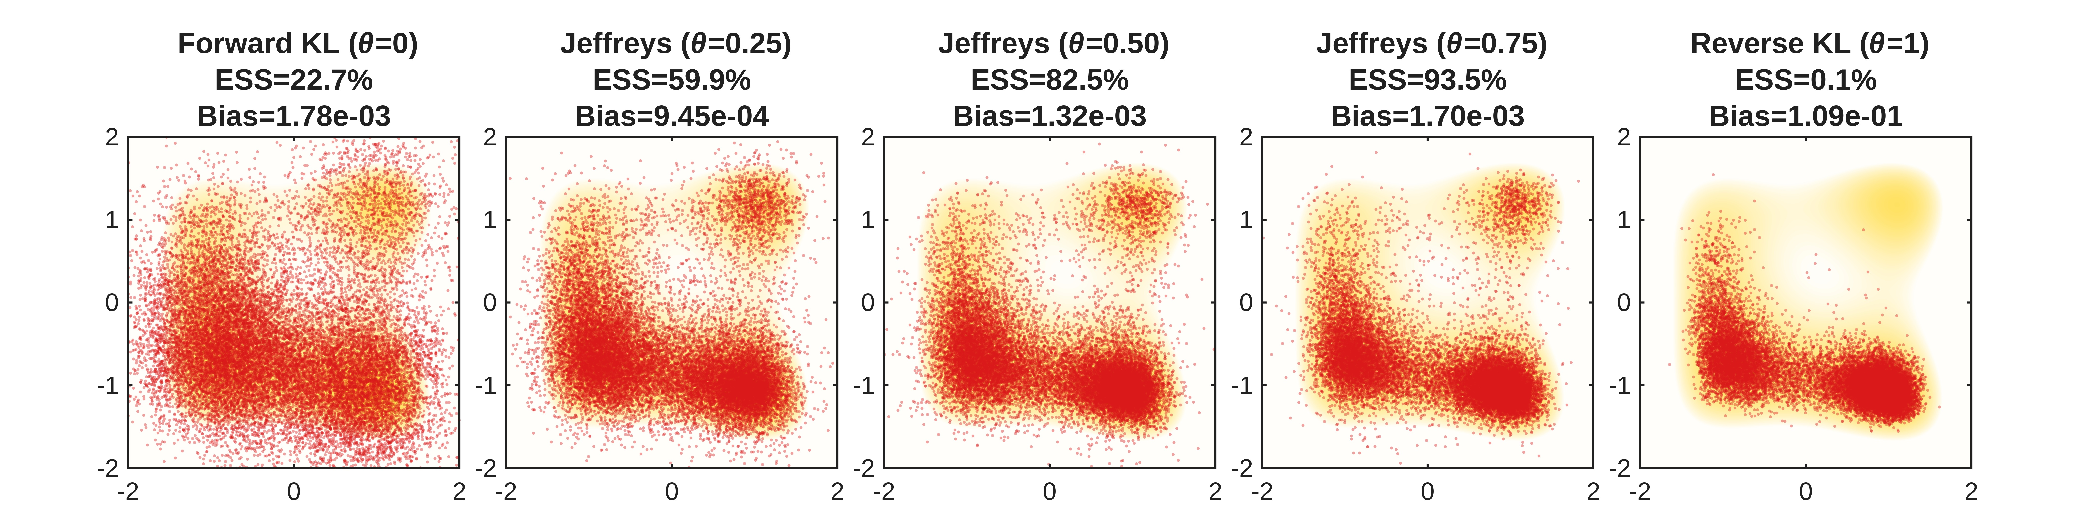
\includegraphics[width=\textwidth]{figures/TW_error.pdf}
	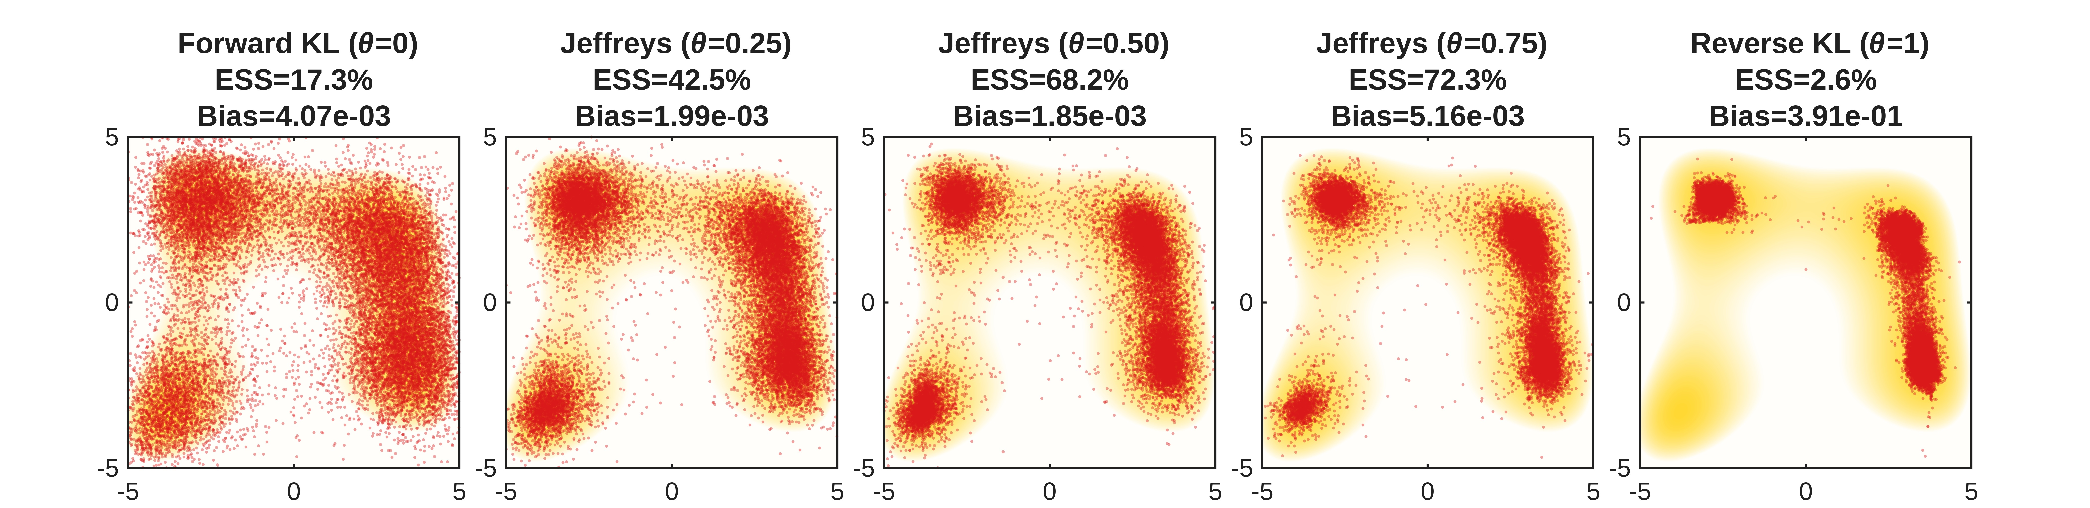
\includegraphics[width=\textwidth]{figures/HB_error.pdf}
	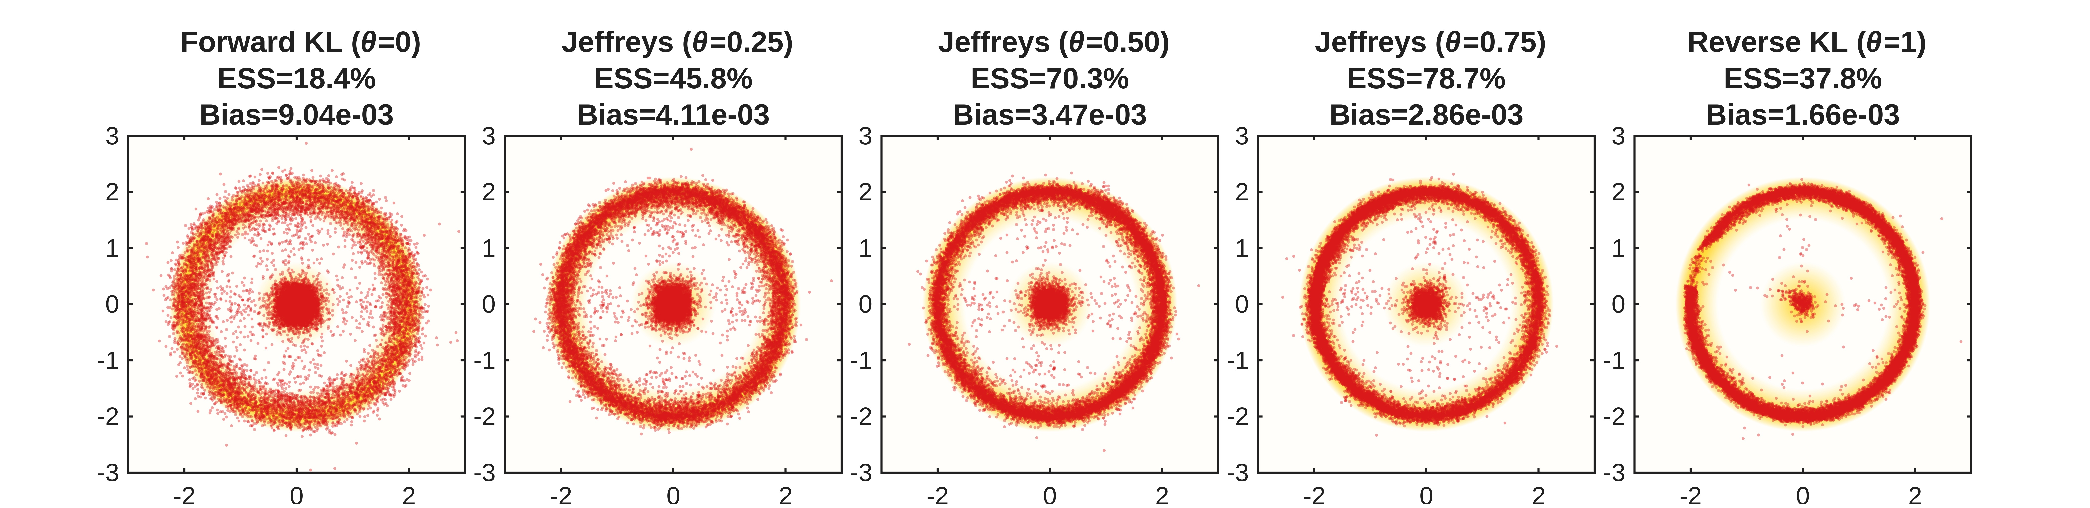
\includegraphics[width=\textwidth]{figures/AN_error.pdf}
	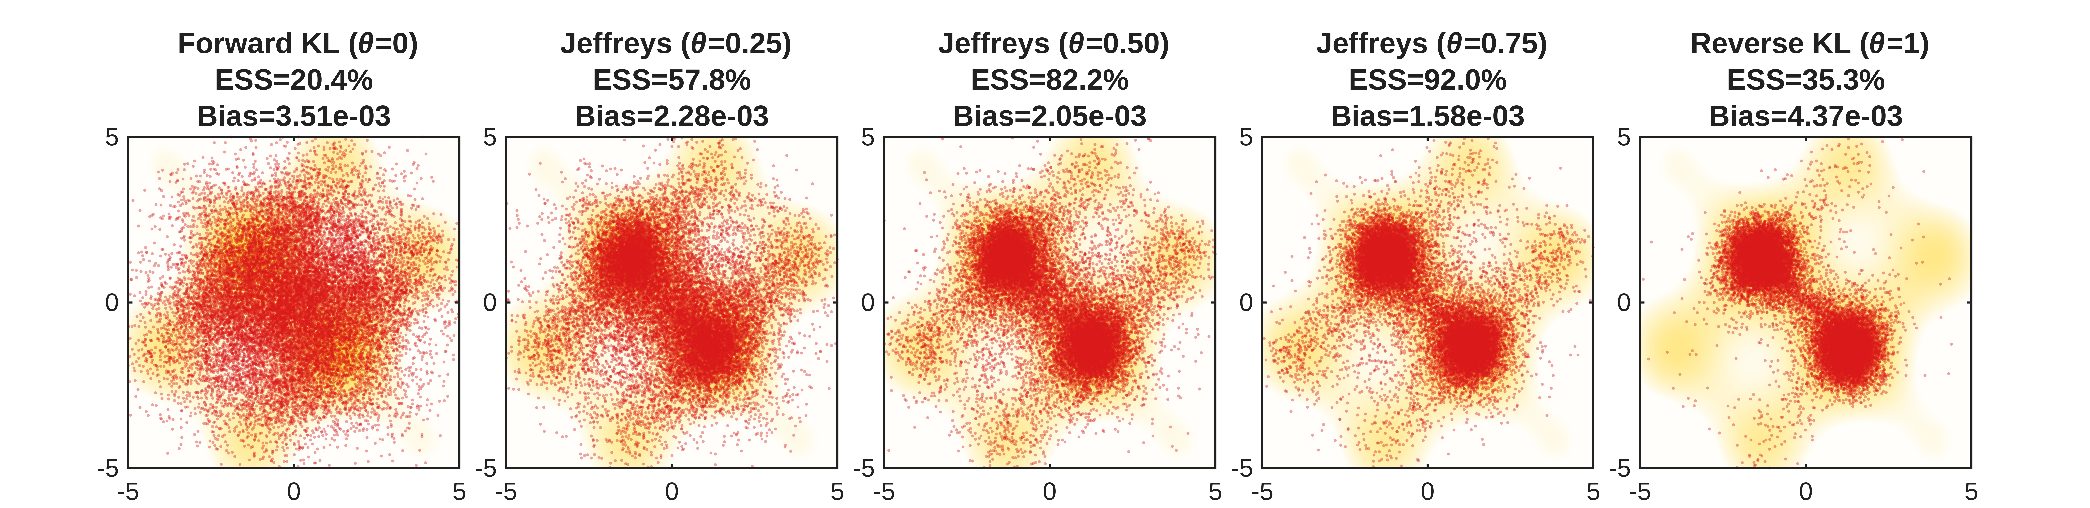
\includegraphics[width=\textwidth]{figures/MW_error.pdf}
	\caption{Density plots of the generated samples across four 2D landscapes. The Jeffreys Flow ($0 < \theta < 1$) robustly corrects the noisy artifacts of Forward KL ($\theta=0$) and strictly prevents the destructive mode collapse inherent to Reverse KL ($\theta=1$).}
	\label{fig: single_step}
\end{figure*}

\begin{figure*}
	\centering
	
\includegraphics[width=\textwidth]{figures/PW_convergence.pdf}
	\caption{Left: The generated distribution from the Jeffreys Flow. The scatter samples accurately capture all modes of the periodic potential ($N=4^{12}$). Right: As sample size $N$ increases, the ESS remains consistently optimal ($\approx 100\%$) while the $L^2$ bias strictly follows the theoretical Monte Carlo convergence rate.}
	\label{fig: single_step_periodic}
\end{figure*}

\begin{figure*}
	\centering
	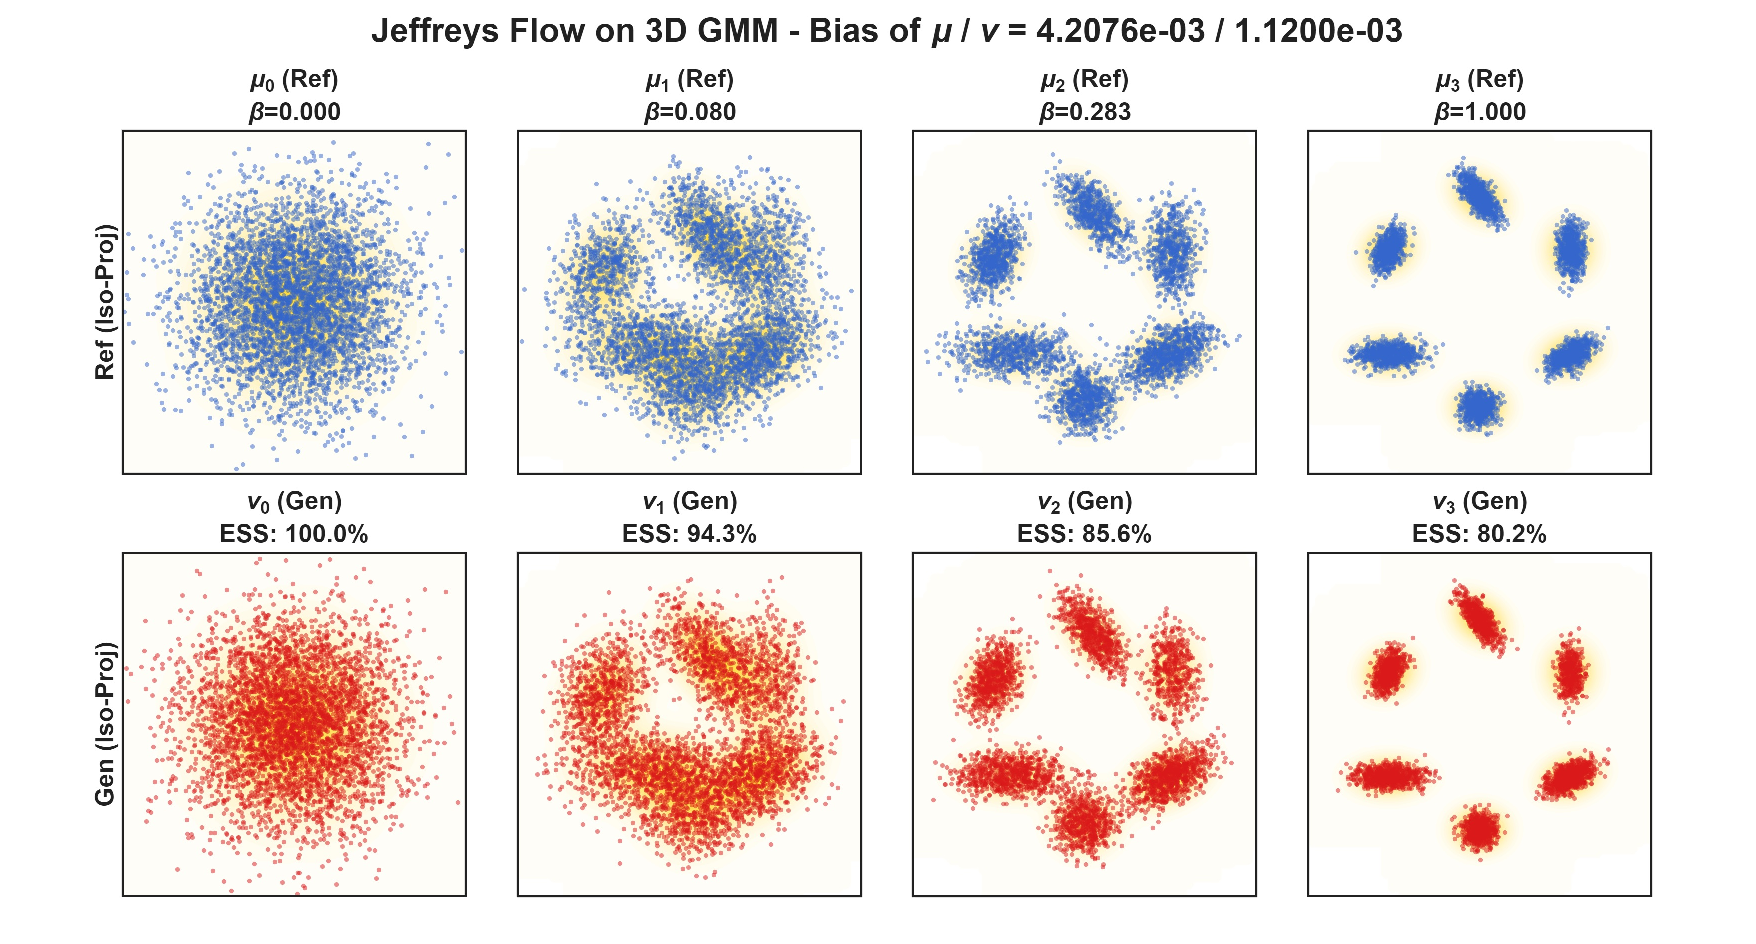
\includegraphics[width=\textwidth]{figures/GM_plot_results.pdf}
	\caption{Sequential distillation on the 3D Gaussian Mixture Model. Top: Reference PT samples at various temperatures. Bottom: Generated samples from the distilled Jeffreys Flow. The resulting bias of the Jeffreys Flow is much smaller than PT.}
	\label{fig: gm_results}
\end{figure*}

\begin{figure*}
	\centering
	
\includegraphics[width=0.9\textwidth]{figures/RB_plot_results.pdf}
	\caption{Sequential distillation on the 4D Rosenbrock. Top: Reference PT samples. Bottom: Generated samples from the Jeffreys Flow successfully learning the highly non-linear correlations.}
	\label{fig: rb_results}
\end{figure*}

\begin{figure*}
	\centering
	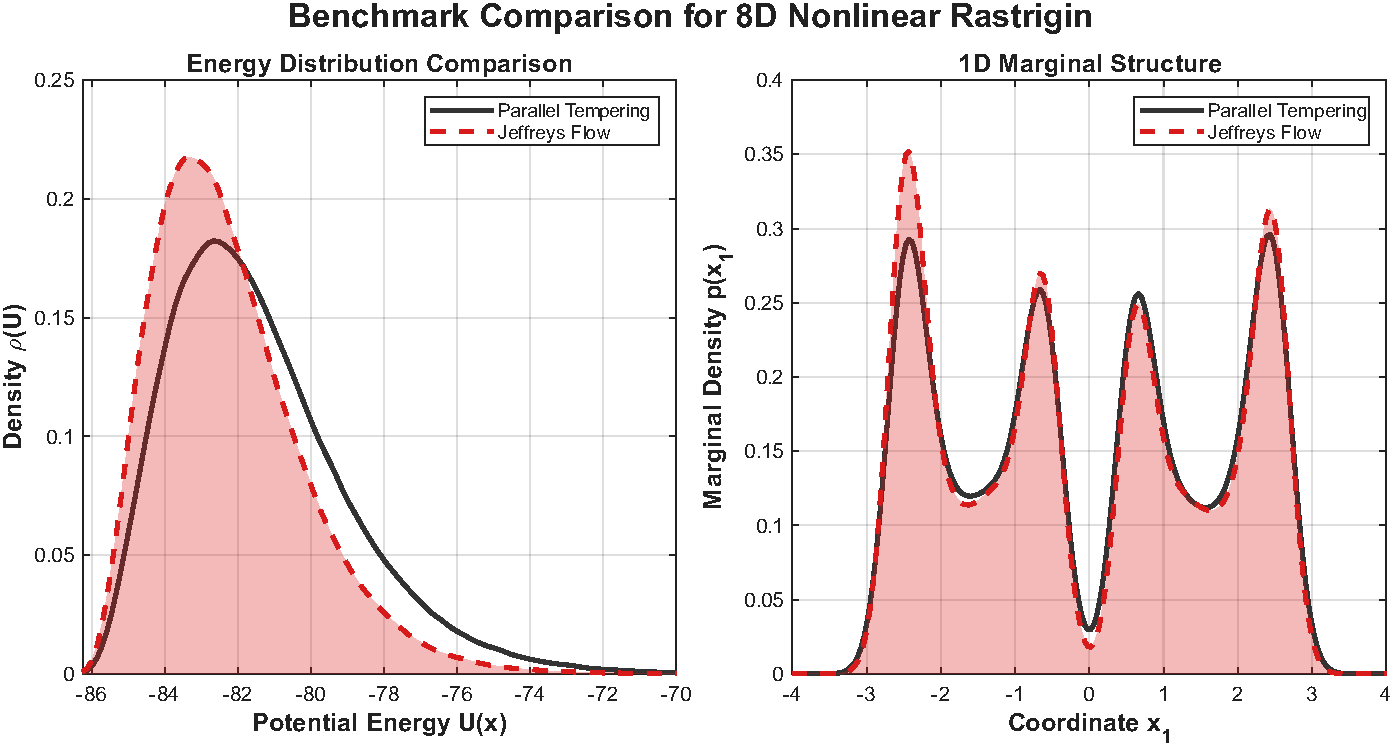
\includegraphics[width=0.9\textwidth]{figures/NR_plot_results.pdf}
	\caption{Comparison for 8D Nonlinear Rastrigin. Left: Potential energy distribution $P(U)$ comparison between PT and Jeffreys Flow. Right: 1D marginal distribution $p(x_1)$ comparison. Both methods show consistent mode coverage and energy profiles.}
	\label{fig: nr_results}
\end{figure*}

\begin{table*}[htbp]
    \centering
    \setlength{\tabcolsep}{4.5pt}
	\setstretch{1.2}
    \begin{tabular}{c |*{11}{c}}
       \hline
       Step & 1 & 2 & 3 & 4 & 5 & 6 & 7 & 8 & 9 & 10 & 11 \\
	   \hline
       $\beta$ & 0.020 & 0.032 & 0.050 & 0.100 & 0.150 & 0.200 & 0.250 & 0.300 & 0.350 & 0.400 & 0.450 \\
       CESS & 94.4\% & 96.1\% & 91.0\% & 78.2\% & 71.5\% & 74.6\% & 82.6\% & 86.7\% & 89.8\% & 92.3\% & 93.4\% \\
       ESS & 94.4\% & 90.7\% & 82.6\% & 64.4\% & \fbox{100\%} & 74.6\% & 61.0\% & 51.9\% & \fbox{100\%} & 92.3\% & 84.7\% \\
       \hline\hline
       Step & 12 & 13 & 14 & 15 & 16 & 17 & 18 & 19 & 20 & 21 & 22 \\
	   \hline
       $\beta$ & 0.500 & 0.550 & 0.600 & 0.650 & 0.700 & 0.750 & 0.800 & 0.850 & 0.900 & 0.950 & 1.000 \\
       CESS & 94.5\% & 95.3\% & 94.5\% & 95.1\% & 95.4\% & 95.5\% & 91.8\% & 94.5\% & 92.0\% & 93.1\% & 85.6\% \\
       ESS & 77.1\% & 68.9\% & 58.9\% & \fbox{100\%} & 95.4\% & 88.1\% & 74.7\% & 61.1\% & \fbox{100\%} & 93.1\% & 74.1\% \\
       \hline 
    \end{tabular}
	\caption{Performance metrics for the 8D Nonlinear Rastrigin potential. The table displays the inverse temperature $\beta$, the CESS, and the ESS at each stage. The ESS is reset to $100\%$ (marked as boxed) whenever adaptive resampling is performed.}
	\label{tab: nr_metrics}
\end{table*}

\begin{figure*}
	\centering
	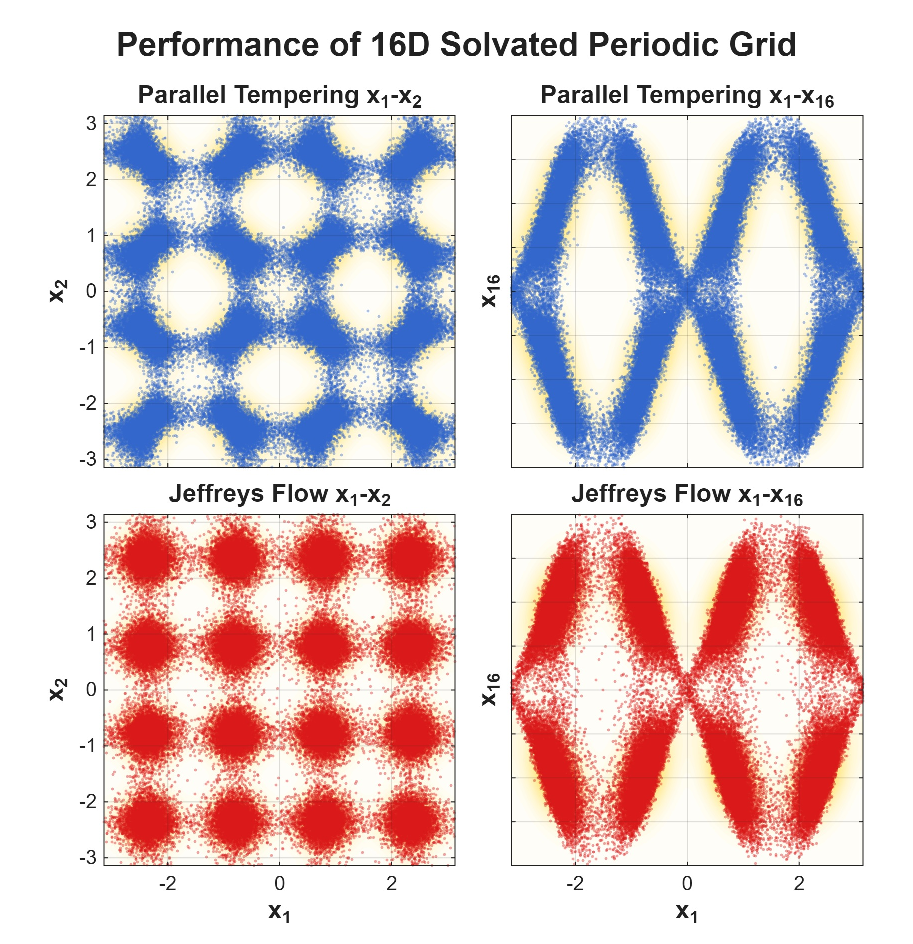
\includegraphics[width=0.6\textwidth]{figures/SL_plot_results_1.pdf}
	\caption{Decorrelation in the 16D Solvated Periodic Grid. Top: PT reference samples exhibit spurious diagonal correlations. Bottom: Jeffreys Flow successfully uncouples the bath to recover the exact independent checkerboard structure.}
	\label{fig: sl_joint}
\end{figure*}

\begin{figure*}
	\centering
	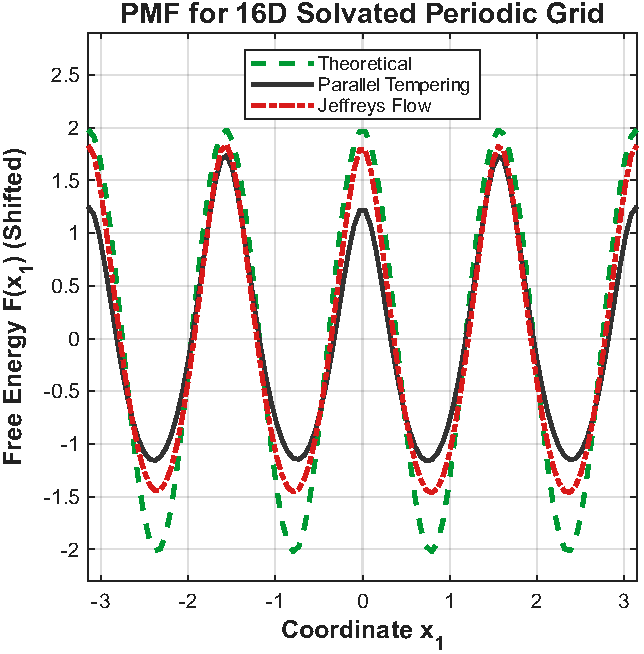
\includegraphics[width=0.5\textwidth]{figures/SL_plot_results_2.pdf}
	\caption{Potential of Mean Force (PMF) along $x_1$. Jeffreys Flow perfectly reconstructs the analytical free energy barriers that PT completely fails to cross.}
	\label{fig: sl_pmf}
\end{figure*}

\begin{figure*}
	\centering
	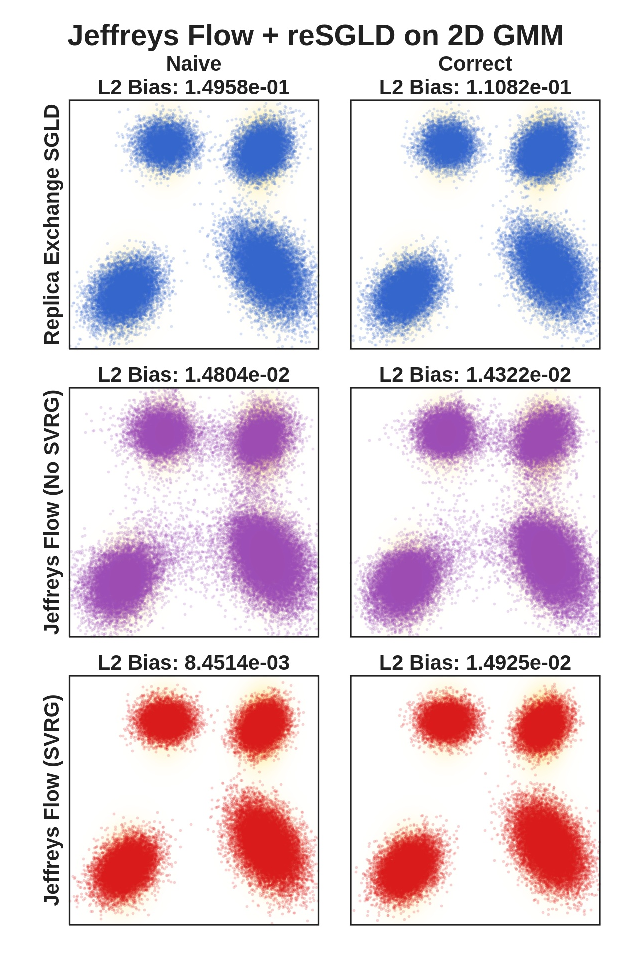
\includegraphics[width=0.5\textwidth]{figures/GM_plot_NU_results.pdf}
	\caption{Decorrelation in the 2D GMM. Visual comparison between reSGLD baselines and Jeffreys Flow configurations. Jeffreys (SVRG) fully resolves the probability density distribution. Jeffreys (No SVRG) generates samples featuring excessive spread and undesirable artificial tails.}
	\label{fig: resgld_results}
\end{figure*}

\begin{table*}[htbp]
    \centering
    \setlength{\tabcolsep}{4.5pt}
	\setstretch{1.2}
    \begin{tabular}{cc |*{6}{c}}
        \hline
        \multicolumn{2}{c|}{Step} & 0 & 1 & 2 & 3 & 4 & 5 \\
        \multicolumn{2}{c|}{$\beta$} & 0.0 & 0.05 & 0.2 & 0.4 & 0.7 & 1.0 \\
        \hline\hline
        reSGLD & Naive & 5.97e-02 & 5.90e-02 & 6.11e-02 & 7.49e-02 & 1.12e-01 & 1.50e-01 \\
        reSGLD & Correct & 9.82e-02 & 3.50e-02 & 4.44e-02 & 6.42e-02 & 9.48e-02 & 1.11e-01 \\
        Jeffreys (No SVRG) & Naive & 2.81e-03 & 2.57e-02 & 1.91e-02 & 1.96e-02 & 1.32e-02 & 1.48e-02 \\
        Jeffreys (No SVRG) & Correct & 4.44e-03 & 9.29e-03 & 8.93e-03 & 1.45e-02 & 1.89e-02 & 1.43e-02 \\
        Jeffreys (SVRG) & Naive & 4.94e-03 & 1.65e-03 & 1.56e-02 & 6.44e-03 & 4.60e-03 & 8.45e-03 \\
        Jeffreys (SVRG) & Correct & 3.75e-03 & 3.08e-03 & 6.87e-03 & 1.05e-02 & 8.22e-03 & 1.49e-02 \\
        \hline
    \end{tabular}
    \caption{Bias Evaluation across the intermediate targets in the 2D GMM experiment. The bias is drastically reduced by training with Jeffreys Flow, filtering out aggressive discretization errors inherent in reSGLD.}
    \label{tab: resgld_bias}
\end{table*}

\begin{table*}[htbp]
    \centering
	\setlength{\tabcolsep}{6pt}
	\setstretch{1.2}
    \begin{tabular}{cc |*{6}{c}}
        \hline
        \multicolumn{2}{c|}{Step} & 0 & 1 & 2 & 3 & 4 & 5 \\
        \multicolumn{2}{c|}{$\beta$} & 0.0 & 0.05 & 0.2 & 0.4 & 0.7 & 1.0 \\
        \hline\hline
        Jeffreys (No SVRG) & Naive & -- & 99.17\% & 97.52\% & 94.42\% & 87.17\% & 76.80\% \\
        Jeffreys (No SVRG) & Correct & -- & 99.16\% & 96.13\% & 93.75\% & 87.51\% & 77.61\% \\
        Jeffreys (SVRG) & Naive & -- & 99.25\% & 96.77\% & 95.34\% & 91.77\% & 86.02\% \\
        Jeffreys (SVRG) & Correct & -- & 98.07\% & 96.80\% & 95.11\% & 91.81\% & 86.64\% \\
        \hline
    \end{tabular}
    \caption{ESS across the intermediate targets in the 2D GMM experiment. High quantitative ESS values demonstrate the ability of Jeffreys Flow as a robust feed-forward Boltzmann Generator for direct, independent sample generation.}
    \label{tab: resgld_ess}
\end{table*}

\begin{table*}[htbp]
	\centering
	\setlength{\tabcolsep}{6pt}
	\setstretch{1.2}
	\begin{tabular}{c |*{8}{c}}
		\hline
		Step & 1 & 2 & 3 & 4 & 5 & 6 & 7 & 8 \\
		\hline\hline
		Exact & 83.93\% & 91.49\% & 92.48\% & 88.69\% & 77.30\% & 85.23\% & 89.56\% & 89.24\% \\
		Full Potential & 83.42\% & 88.28\% & 93.09\% & 88.83\% & 79.90\% & 86.18\% & 89.25\% & 91.15\% \\
		Stochastic & 61.71\% & 64.27\% & 84.69\% & 90.00\% & 89.08\% & 93.23\% & 79.66\% & 94.14\% \\
		\hline
	\end{tabular}
	\caption{CESS across the intermediate targets in the 2D Screened Poisson experiment. All evaluated configurations sustain extremely high CESS scores, confirming the robustness and massive acceleration achieved by the trained Jeffreys Flow.}
	\label{tab: poisson_ess}
\end{table*}

\begin{figure*}
	\centering
	
\includegraphics[width=\textwidth]{figures/P_plot_Poisson_Setup.pdf}
	\caption{2D Screened Poisson Equipment Setup. Left: The true multi-source distribution field generated by the ground truth locations. Right: The resulting physical response $u(x)$ modeled by solving the discretized Poisson PDE. The $81$ fixed local sensors (square markers) collect the noisy measurements used to infer the unknown source locations (star markers).}
	\label{fig: poisson_setup}
\end{figure*}

\begin{figure*}
	\centering
	
\includegraphics[width=0.75\textwidth]{figures/P_plot_MU_NU_results.pdf}
	\caption{Marginal Posterior for Source 1 ($\theta_1$) in the Poisson Inverse Problem. The Exact configuration produces tightly bounded, high-fidelity posterior samples. The Neural Network-approximated Stochastic result exhibits structural degradation, validating the necessity of using exact PDE evaluations for calculating the importance weights.}
	\label{fig: poisson_marginals}
\end{figure*}

\begin{table*}[htbp]
	\centering
	\setlength{\tabcolsep}{6pt}
	\setstretch{1.2}
	\begin{tabular}{c |*{7}{c}}
		\hline
		Discretization $N$ & 8 & 12 & 16 & 20 & 24 & 28 & 32 \\
		\hline\hline
		$L^2$ Bias & 1.60e-02 & 7.45e-03 & 5.93e-03 & 3.56e-03 & 4.02e-03 & 2.00e-03 & 3.84e-04 \\
		\hline
	\end{tabular}
	\caption{Sampling Bias Evaluation in High Dimensions. Using solely a single transport map trained exclusively at the truncated dimension $N_0 = 8$, the reweighted Jeffreys Flow generates high-fidelity sampling accuracy uniformly up to $N = 32$, with the bias adhering to the rapid theoretical $\mathcal{O}(1/N^2)$ discretization error decay.}
	\label{tab: pimc_bias}
\end{table*}

\begin{figure*}
	\centering
	
\includegraphics[width=0.6\textwidth]{figures/compare_MU_S1_S2.pdf}
	\caption{Quantum Path Integral Distillation. Comparison of the marginal spatial density between the classical distribution constructed from the empirical training samples and the distilled quantum distribution extracted using Jeffreys Flow.}
	\label{fig: pimc_density}
\end{figure*}

\begin{figure*}
	\centering
	
\includegraphics[width=0.6\textwidth]{figures/compare_CESS_S1_S2.pdf}
	\caption{Progression of the CESS over the intermediate bridging steps. Sustained high CESS scores confirm the robustness and stability of the transport map during the classical-to-quantum distillation sequence.}
	\label{fig: pimc_cess}
\end{figure*}

\end{document}
